\chapter{The Tokai to Kamioka Experiment}
\label{chap:detectors}
The Tokai to Kamioka (T2K) experiment in Japan was proposed and designed in the early to mid 2000s with the intent of observing electron neutrino appearance, alongside precision measurement of muon neutrino disappearance\cite{t2k_loi,t2k_prop}. In 2014 T2K were first to observe electron neutrino appearance, finding a larger mixing angle $\sin^2\theta_{13}$ than measured by the reactors\cite{t2k_disc}. NO$\nu$A confirmed the appearance measurement in 2016\cite{nova_disc}, finding similar values of $\sin^2\theta_{13}$.

The current effort in the $\nu_\mu \rightarrow \nu_e$ channel is reducing the allowed phase space of the CP violating Dirac phase, $\delta_{CP}$, and continuing the measurements of $\sin^2 \theta_{13}$. Including the  $\nu_\mu \rightarrow \nu_e$ channel(s) also significantly reduces $\sin^2 \theta_{23}$ uncertainties\cite{nova_neutrino2018}. In the muon disappearance measurements, T2K is comparing neutrino and anti-neutrino oscillation parameters and seeing indications of normal neutrino mass ordering\cite{t2k_2017}.
\begin{figure}[h]
	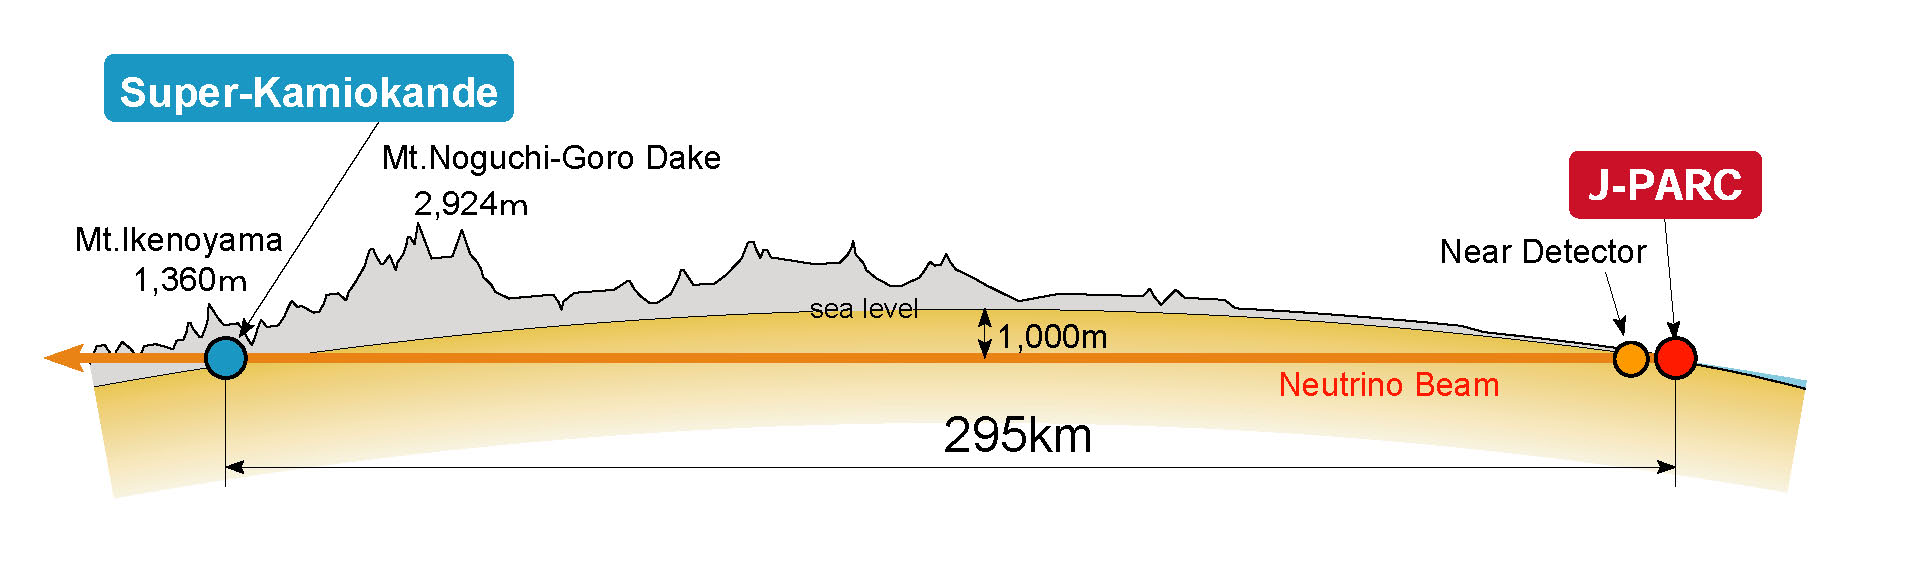
\includegraphics[width=1.0\textwidth, trim={0mm 0mm 0mm 0mm}, clip,page=1]{figures/det_chap/view/t2k_overview}
	\caption{The T2K experiment where neutrinos are created at the J-PARC complex in Tokai. The neutrino beam is characterised at the near-detectors 280 m downstream. 295 km west is the Super-Kamiokande far-detector, measuring the oscillated neutrino spectrum}
	\label{fig:t2k_overview}
\end{figure}

The neutrinos at T2K are born from particle decay---primarily $K^\pm$, $\pi^\pm$ and $\mu^\pm$---after a proton beam impinges on a target at the J-PARC complex on the Japanese coast, $\sim 120\text{ km}$ north east of Tokyo. The neutrino beam is measured by the ND280 and INGRID detectors $\sim280$ m downstream of the target and a muon monitor station, which provide information on the neutrino flux, directionality and interaction cross-section. The far detector, Super-Kamiokande, sits 295 km downstream of the target station and measures the rate of neutrino interactions on its 50,000 tonnes of purified water, detailed in \autoref{sec:sk}. A schematic of the neutrinos' travel is shown in \autoref{fig:t2k_overview}.
\begin{figure}[h]
	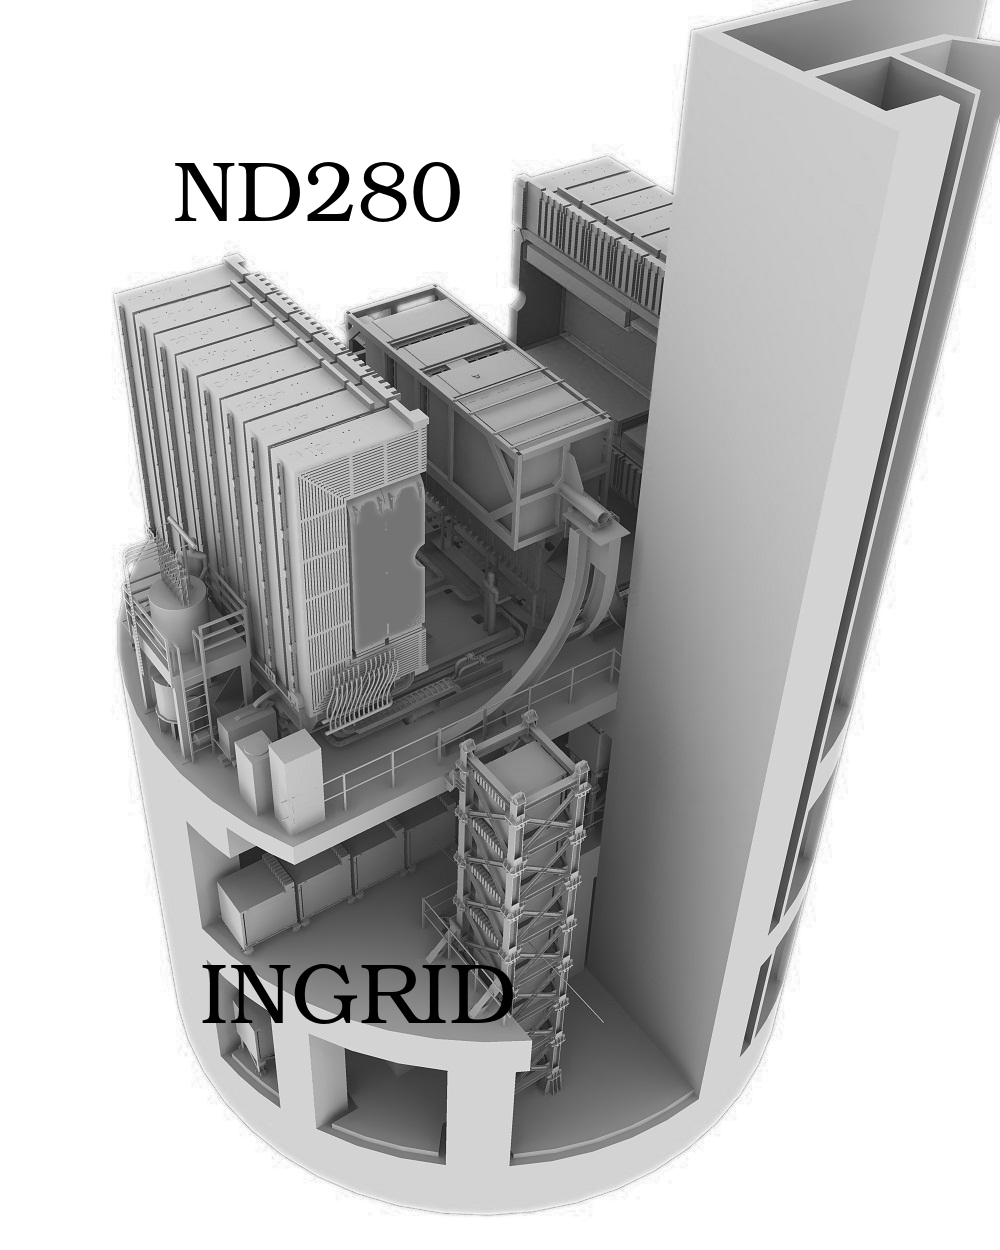
\includegraphics[width=0.4\textwidth, trim={10mm 0mm 0mm 0mm}, clip,page=1]{figures/det_chap/view/image_nd.jpeg}
	\caption{The suite of near-detectors at 280 m from the target, showing ND280 and INGRID}
\end{figure}

A host of other neutrino detectors---not used in this analysis---sit in the same ``pit'' 280 m from the target station as ND280 and INGRID. Examples include the liquid emulsion NINJA experiment\cite{ninja}, the water target WAGASCI\cite{wagasci} experiment and its magnetic calorimeter Baby-MIND\cite{baby_mind}.

\section{Beamline}
The J-PARC complex\cite{jparc_tdr} is used to accelerate protons to 30 GeV/c using a linear accelerator (LINAC), a rapid cycling synchrotron (RCS) and a main ring (MR) synchrotron. The MR has the ability to fast-extract into the neutrino beamline with a design power of 750 kW with proton momentum of 30 GeV/c, using $\sim3\times10^{14}$ protons per spill with 8 proton bunches per spill and a spill cycle of $\sim0.5$ Hz. The spill width, which opens the trigger window at the neutrino detectors, is $\sim5 \mu$s\cite{t2k_det}.
\begin{figure}[h]
	\begin{subfigure}[t]{0.4\textwidth}
		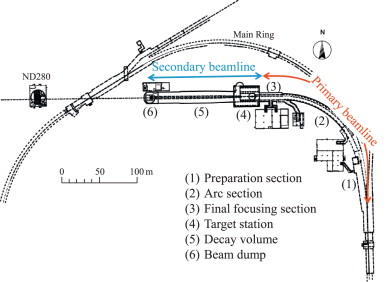
\includegraphics[width=\textwidth, trim={0mm 0mm 0mm 0mm}, clip,page=1]{figures/det_chap/beam/beam.jpg}
		\caption{Top-view}
	\end{subfigure}
	\begin{subfigure}[t]{0.4\textwidth}
		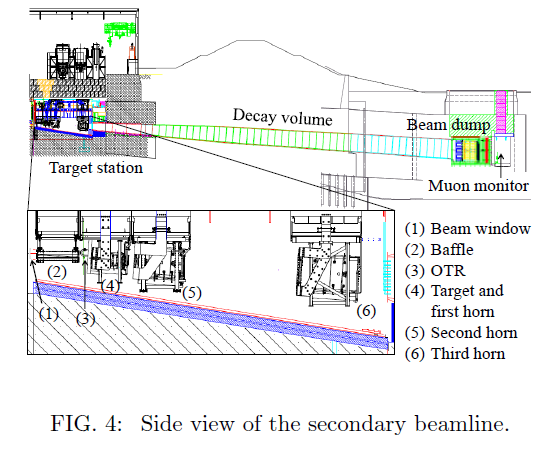
\includegraphics[width=\textwidth, trim={0mm 18mm 0mm 0mm}, clip,page=1]{figures/det_chap/beam/sideview_beam}
		\caption{Side-view of target-dump section}
	\end{subfigure}
	\caption{The neutrino beamline for neutrinos at J-PARC}
	\label{fig:neutrino_beamline}
\end{figure}

The neutrino beamline consists of two parts and is shown in \autoref{fig:neutrino_beamline}: the primary beamline---which takes fast-extracted protons from the MR, bends them to point towards SK, and impinges them on a graphite target---and the secondary beamline---which directs the mesons from the proton-target interaction through a decay volume, finishing with a beam dump. Shortly after the target in the secondary beamline are three magnetic horns\cite{t2k_horns} which are used to deflect (focus) wrong-sign (right-sign) mesons to reduce wrong-sign and enhance right-sign neutrinos. Running the magnets at 250 kA (1.7 T) increases the neutrino flux at SK by factor $\sim17$\cite{t2k_beam}. Taking data in $\nu_\mu$ dominated mode is referred to as Forward Horn Current (FHC) mode, and in $\bar{\nu}_\mu$ dominated mode as Reverse Horn Current (RHC) mode. The focused mesons pass through a $\sim96$ m decay volume in which the majority of them decay. Remaining particles then strike the beam dump, which stops all mesons. Surviving high momentum muons ($p_\mu > 5.0 \text{ GeV/c}$) generally pass through the beam dump, after which they are measured by muon monitors. The MUMON muon monitors (one ionisation chamber and one silicon PIN photodiode) infer the neutrino beam direction to better than 0.25 mrad and the beam intensity better than 3\%\cite{t2k_mumon,t2k_mumon2}, and are used to inform the beam simulation group.

The neutrinos come primarily from three meson decays
\begin{align*}
	\pi^+ & \rightarrow \mu^+ + \nu_\mu 		&  99.99\% 			& & K^+ & \rightarrow \mu^+ + \nu_\mu 			& 63.6\% & & K^0_L & \rightarrow \pi^- + e^+ + \nu_e 	  & 40.6\% \\
	      & \rightarrow e^+ + \nu_e 			&  10^{-4}\%		& &		& \rightarrow \pi^0 + e^+ + \nu_e 		& 5.1\%  & &	   & \rightarrow \pi^- + \mu^+ + \nu_\mu &  27.0\% \\
	      & \rightarrow \mu^+ + \nu_\mu + \gamma & 2\times 10^{-4}\%  & &		& \rightarrow \pi^0 + \mu^+ + \nu_\mu  	& 3.5\%  & &	   & & 		 &
\end{align*}

\iffalse
\begin{align*}
	\pi^+ 	& \rightarrow \mu^+ + \nu_\mu & 0.9999\\
			& \rightarrow e^+ + \nu_e 	  & 0.0001\\
	K^+   	& \rightarrow \mu^+ + \nu_\mu & 0.6355\\
			& \rightarrow \pi^0 + \mu^+ + \nu_\mu & 0.0353\\
			& \rightarrow \pi^0 + e^+ + \nu_e & 0.0507\\
	K^0_L 	& \rightarrow \pi^- + \mu^+ + \nu_\mu & 0.2704\\
			& \rightarrow \pi^- + e^+ + \nu_e & 0.4055
\end{align*}
\fi
and one leptonic decay\cite{pdg_2017}
\begin{align*}
\mu^+ \rightarrow e^+ + \bar{\nu}_\mu + \nu_e & & 100\%
\end{align*}

From the beam simulation we trace back each neutrino's parent meson, shown in \autoref{fig:flux_parents}. The $\pi$ parent is clearly dominant for both the \numu and \numubar fluxes, although the portion with $E_\nu > 3\text{ GeV}$ consists of neutrinos whose parents are $K$ mesons. The \nue and \nuebar components of the neutrino beam come primarily from the leptonic $\mu$ decay below $E_\nu = 1 \text{ GeV}$ and from $K^+$ and $K^0_L$ at $E_\nu = 2 \text{ GeV}$. Tertiary decay products, e.g. a $\pi^-$ from a $K^0_L$ decay, form large portions of the wrong-sign background.
\begin{figure}[h]
	\begin{subfigure}[t]{0.32\textwidth}
		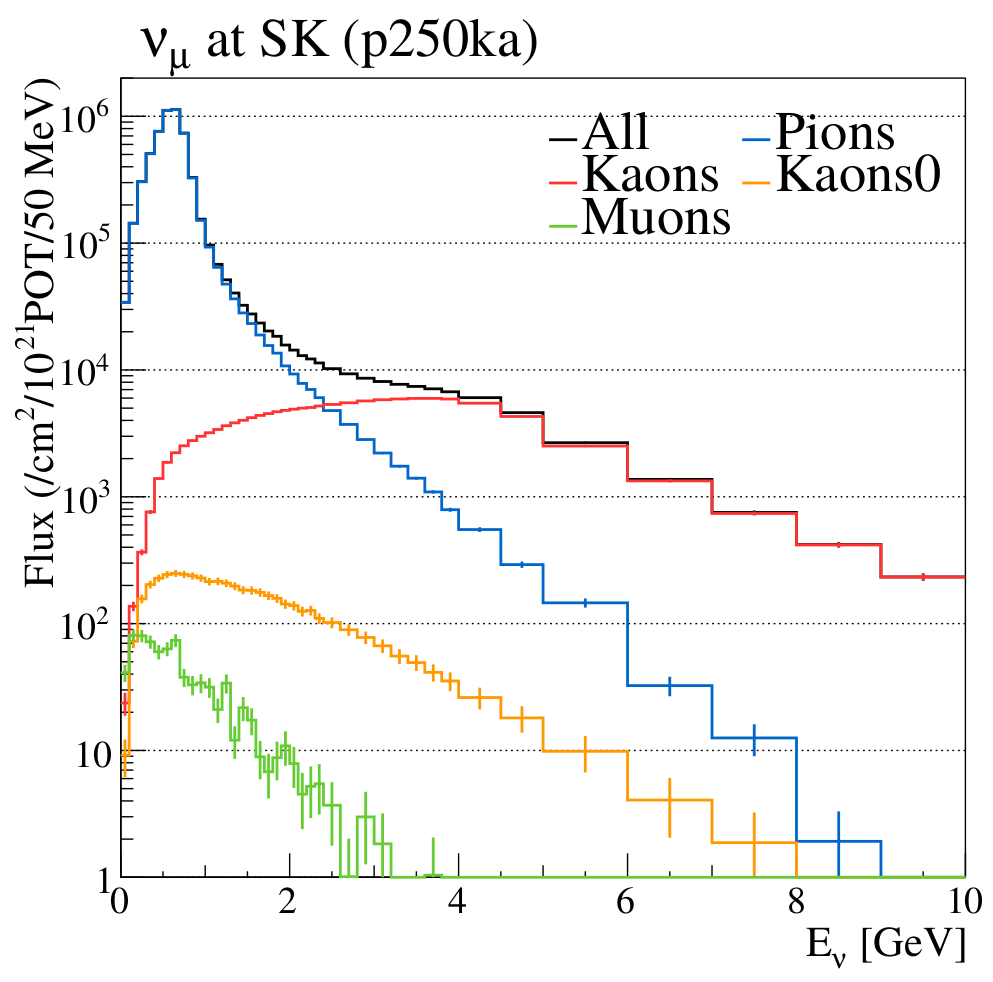
\includegraphics[width=\textwidth, trim={0mm 0mm 0mm 0mm}, clip,page=1]{figures/det_chap/beam/numu_sk_parents}
	\end{subfigure}
	\begin{subfigure}[t]{0.32\textwidth}
		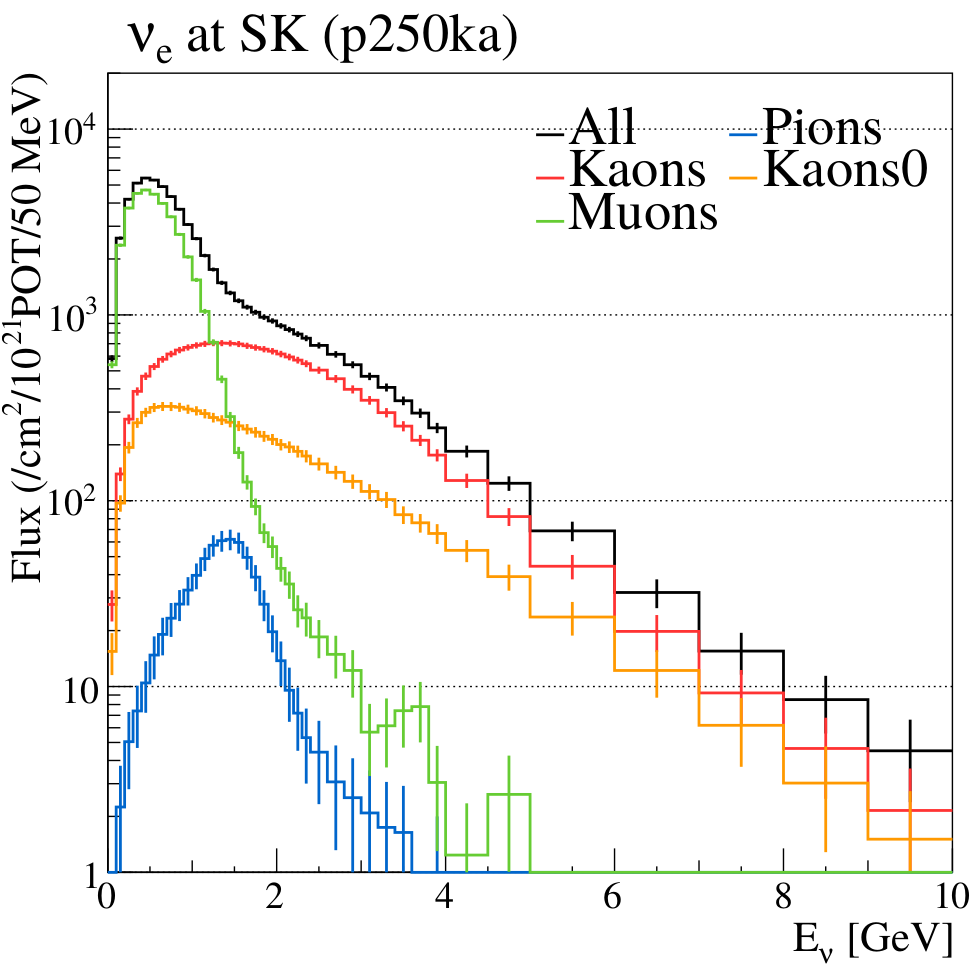
\includegraphics[width=\textwidth, trim={0mm 0mm 0mm 0mm}, clip,page=1]{figures/det_chap/beam/nue_sk_parents}
	\end{subfigure}

	\begin{subfigure}[t]{0.32\textwidth}
		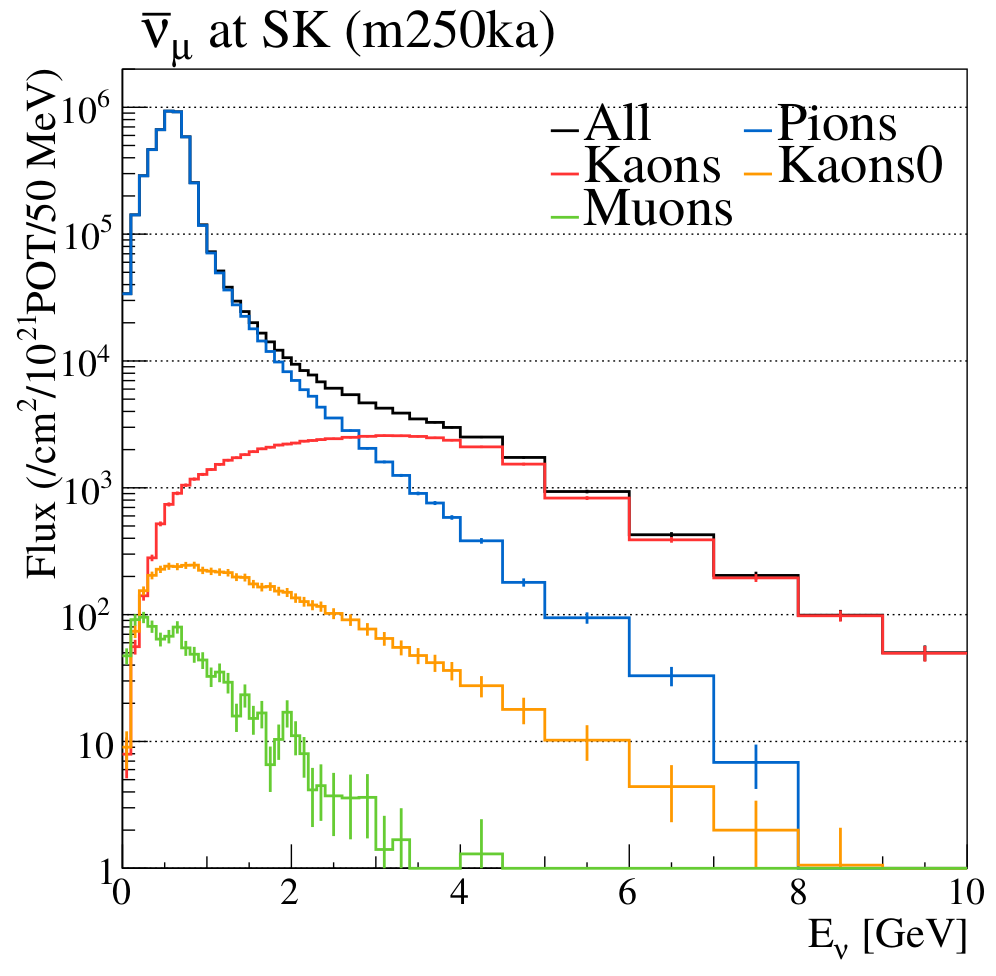
\includegraphics[width=\textwidth, trim={0mm 0mm 0mm 0mm}, clip,page=1]{figures/det_chap/beam/numubar_sk_parents}
	\end{subfigure}
	\begin{subfigure}[t]{0.32\textwidth}
		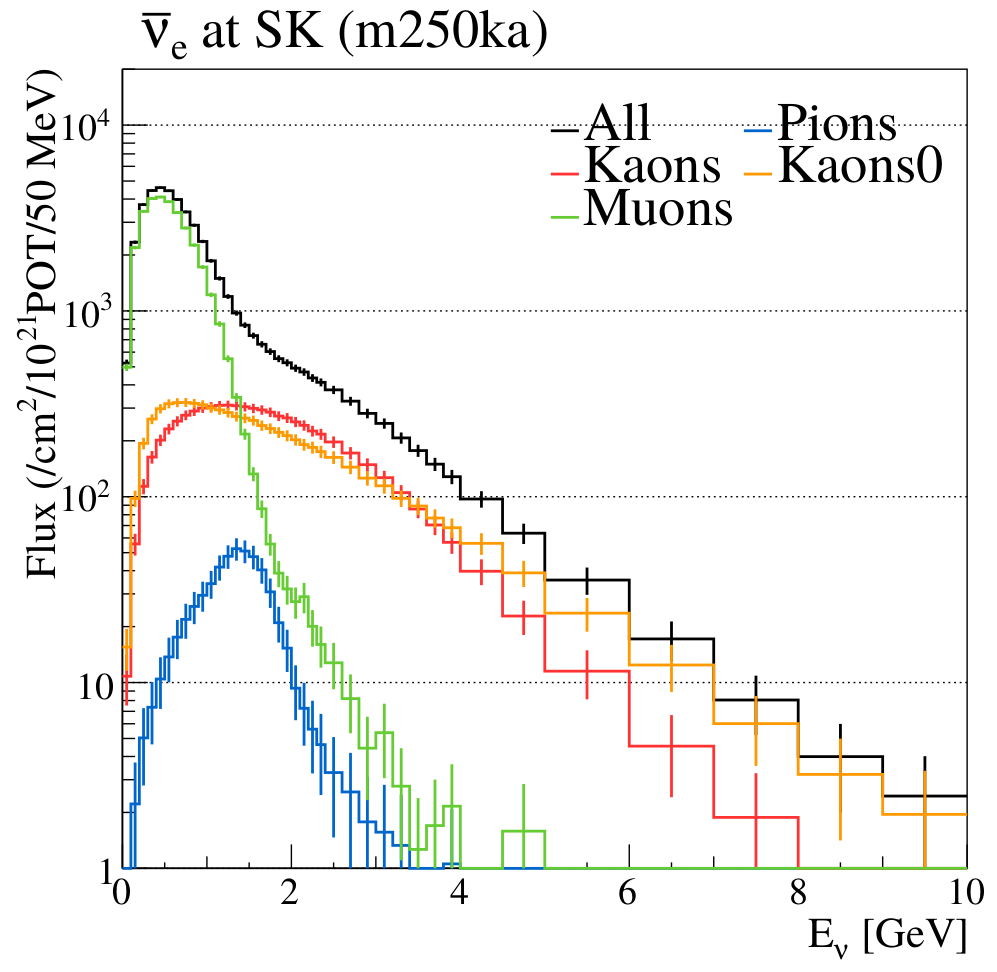
\includegraphics[width=\textwidth, trim={0mm 0mm 0mm 0mm}, clip,page=1]{figures/det_chap/beam/nuebar_sk_parents}
	\end{subfigure}
	\caption{Simulated right-sign neutrino fluxes at SK, showing parents}
	\label{fig:flux_parents}
\end{figure}

T2K was the first long baseline accelerator experiment to use the ``off-axis technique'' in which the far-detector is offset from the neutrino beam center\cite{off_axis}. This has two main effects: 1) it focuses the neutrino energy spectra into a narrower ``peak'' (albeit with lower overall rate than on-axis), and 2) it reduces the wrong-sign background for $\nu_e$ appearance searches. Assuming the neutrino parents are solely charged pions from $\pi^+\rightarrow\mu^+\nu_\mu$, we can approximate the neutrino energy $E_\nu$ as a function of pion-neutrino angle $\theta_{\pi,\nu}$ (colloquially ``off-axis angle''), pion energy $E_\pi$ and mass $m_\pi$, and the muon mass $m_\mu$,
\begin{equation}
	E_\nu = \frac{m^2_\pi-m^2_\mu}{2\left( E_\pi - p_\pi \cos \theta_{\pi,\nu} \right)} 
\end{equation}

For a chosen $\cos \theta_{\pi,\nu}$ there is a maximum pion energy of $E_\pi^\text{max} = p_\pi/\cos\theta_{\pi,\nu}$ giving rise to a maximum neutrino energy of
\begin{equation}
	E_\nu^\text{max} = \frac{m^2_\pi-m^2_\mu}{2E_\pi \sin^2 \theta_{\pi,\nu}} 
\end{equation}

\noindent which maximises when $\pi$ and $\nu$ approach collinearity, and as $\theta$ increases the allowed neutrino energy spectrum becomes smaller. The calculated flux at SK with the neutrino oscillation probability is shown in \autoref{fig:off-axis}. The off-axis angle is chosen to maximise the flux in the primary oscillation dip at $E_\nu \sim 0.6\text{ GeV}$.
\begin{figure}[h]
	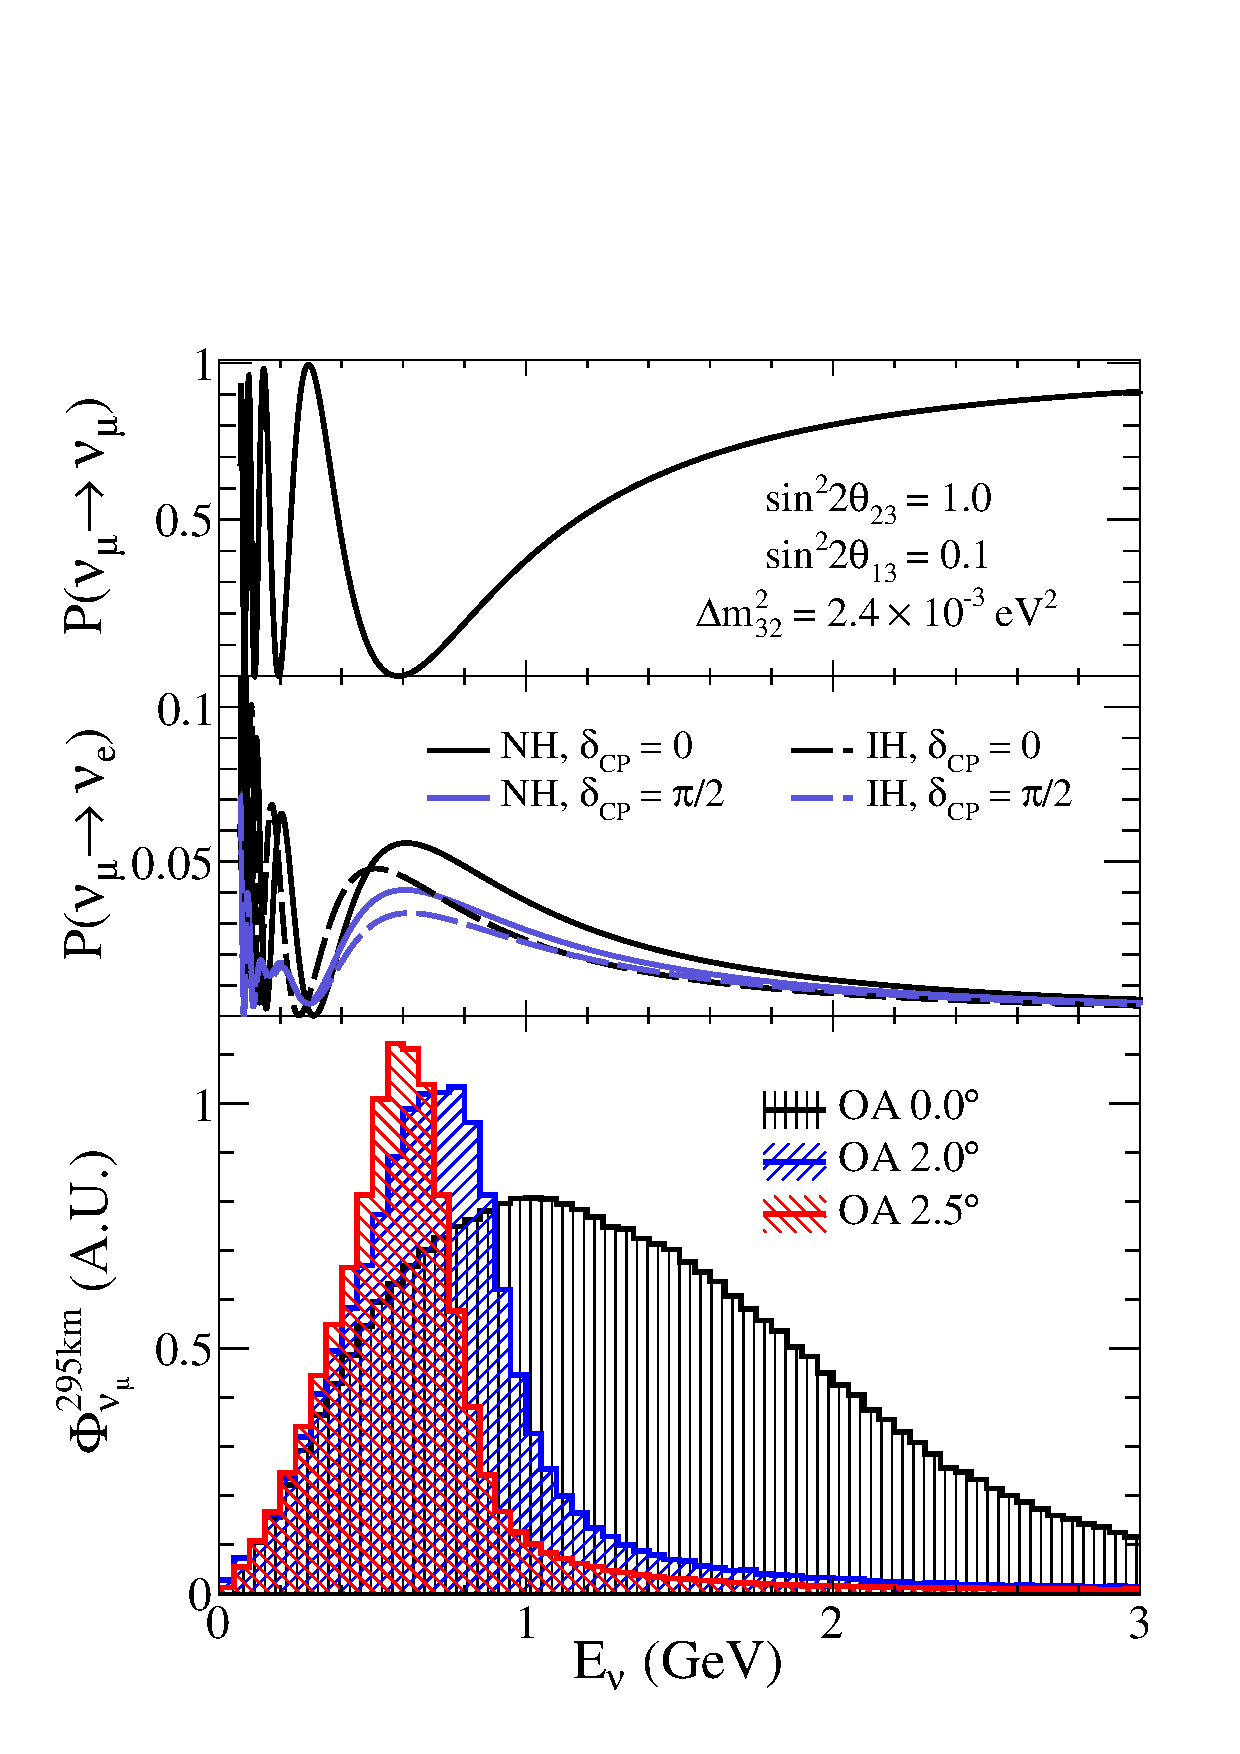
\includegraphics[width=0.4\textwidth, trim={0mm 0mm 0mm 0mm}, clip,page=1]{figures/det_chap/oaeffect_pnue_pnumu_flux}
	\caption{Effect of off-axis (OA) angle on the SK neutrino flux}
	\label{fig:off-axis}
\end{figure}

The delivered beam power and accumulated POT has been steadily increasing from run 1 in 2010 to run 9 in 2019. Run 9 concluded with $\sim500\text{ kW}$ beam power, accumulating a total POT of $\sim3.16\times 10^{21}$\footnote{Or 5.28 mg of protons}: $1.51\times 10^{21}$ in FHC and $1.65\times 10^{21}$ in RHC modes.
\begin{figure}[h]
	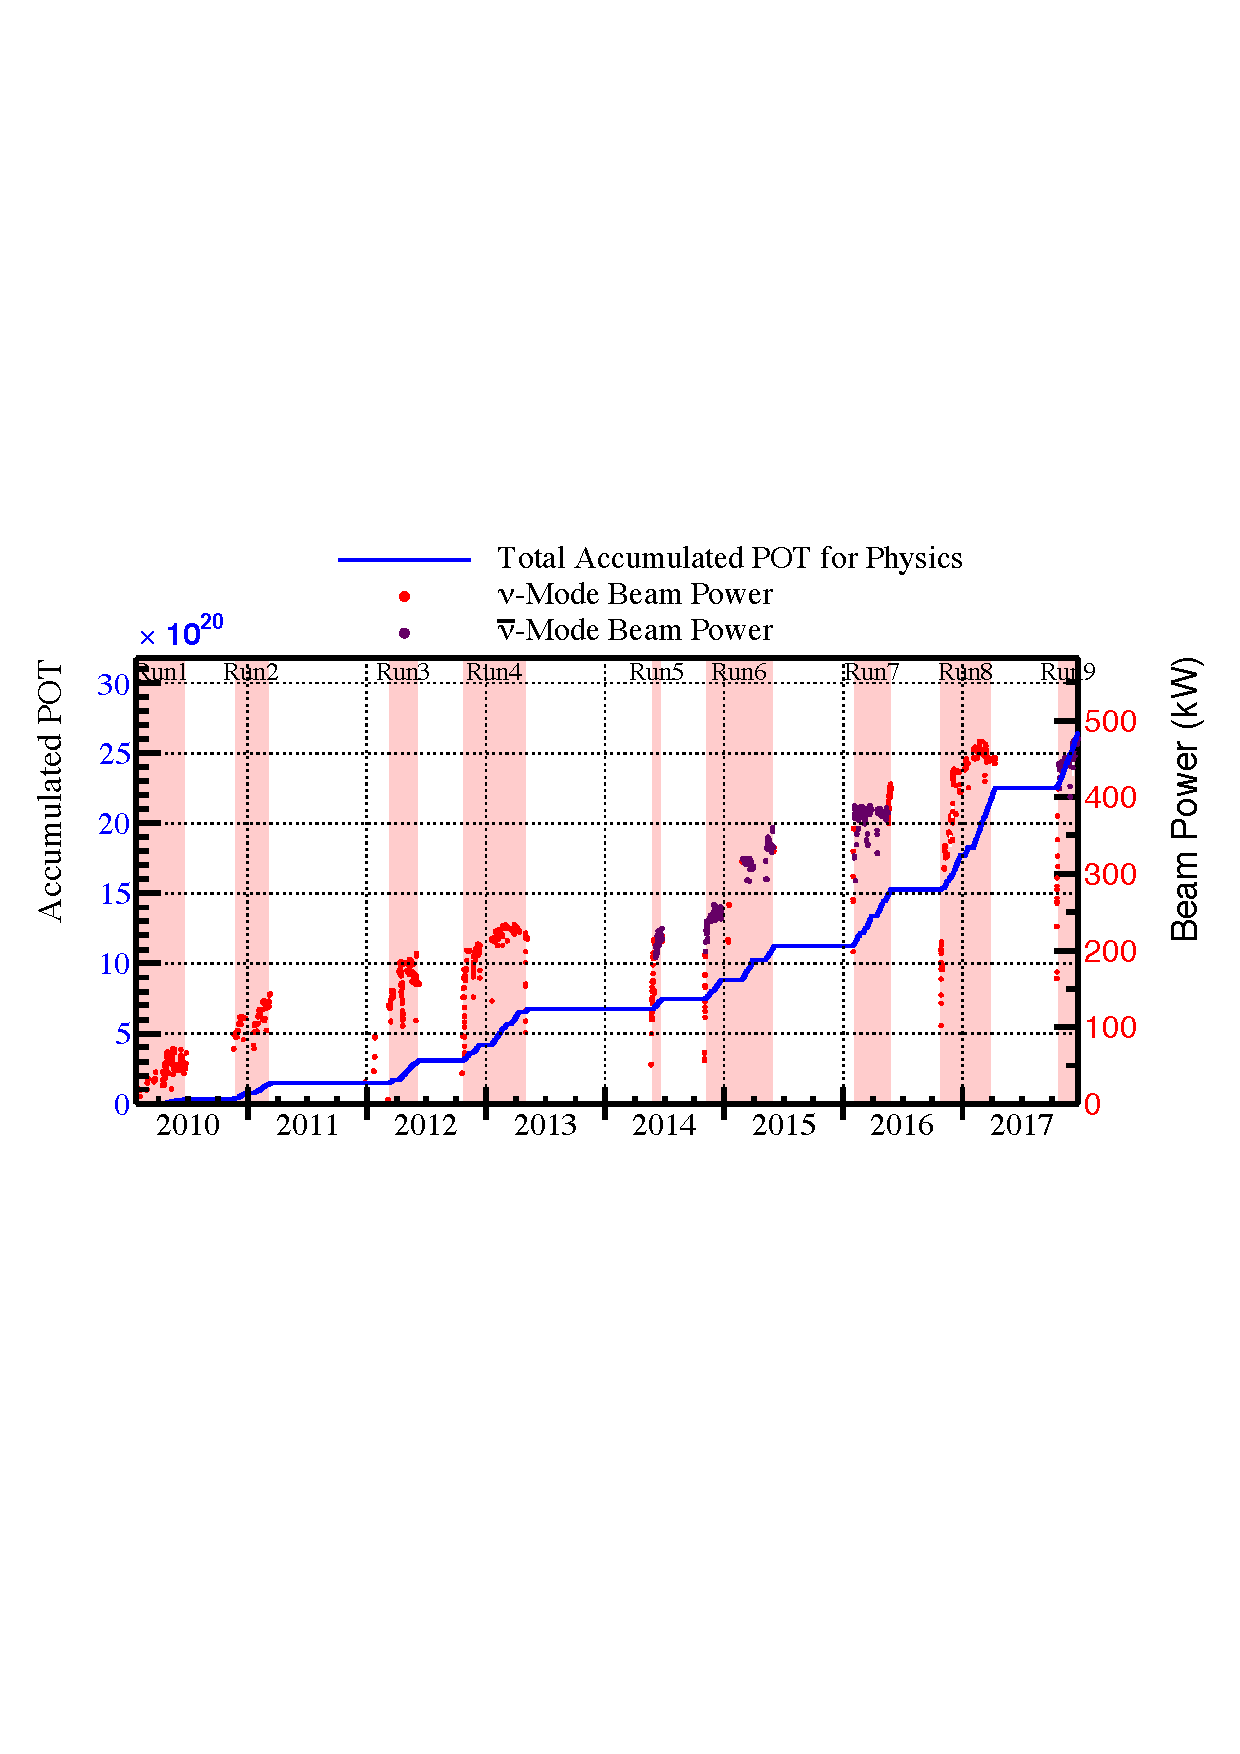
\includegraphics[width=0.5\textwidth, trim= {7mm 40mm 7mm 12mm}, clip]{{figures/pow_t2k_all_toRun77full}}
	\caption{T2K protons on target and beam power for run 1-9}
	\label{fig:t2k_pot}
\end{figure}

The final simulated neutrino fluxes for run 2 to 8 at ND280 are shown in \autoref{fig:flux_1to8}. The wrong-sign background in FHC is $\sim18\%$ at the flux peak which reduces further due to the lower anti-neutrino interaction cross-section, and the \nue component is less than 1\% in the flux peak. The right-sign flux in RHC is similar to the \numu in FHC, and the majority of the contamination of \numu events in RHC mode comes from the higher \numu cross-section rather than the flux.
\begin{figure}[h]
	\begin{subfigure}[t]{0.45\textwidth}
		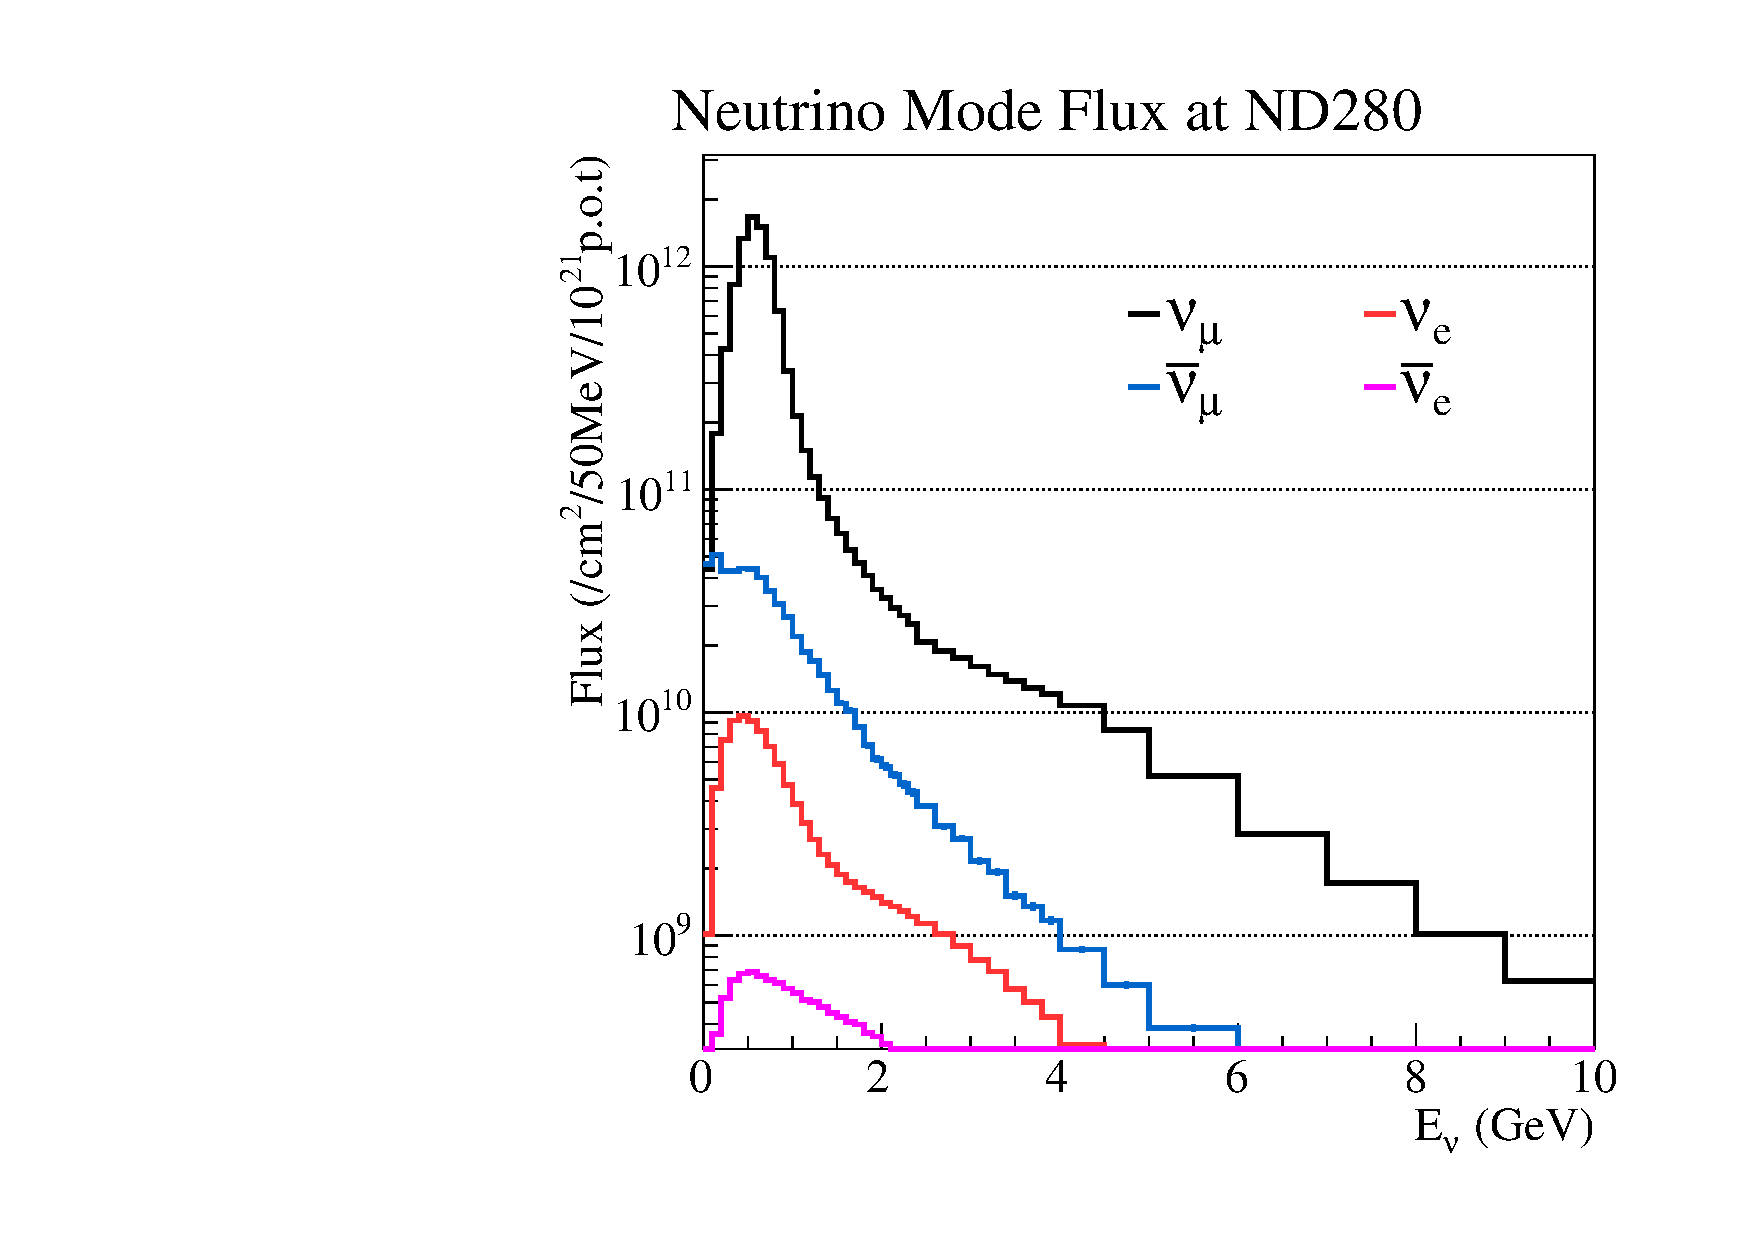
\includegraphics[width=\textwidth, trim={0mm 0mm 0mm 0mm}, clip,page=1]{figures/det_chap/beam/nd5_alltunedflux_run1-8_zoomed_13a}
		\caption{FHC}
	\end{subfigure}
	\begin{subfigure}[t]{0.45\textwidth}
		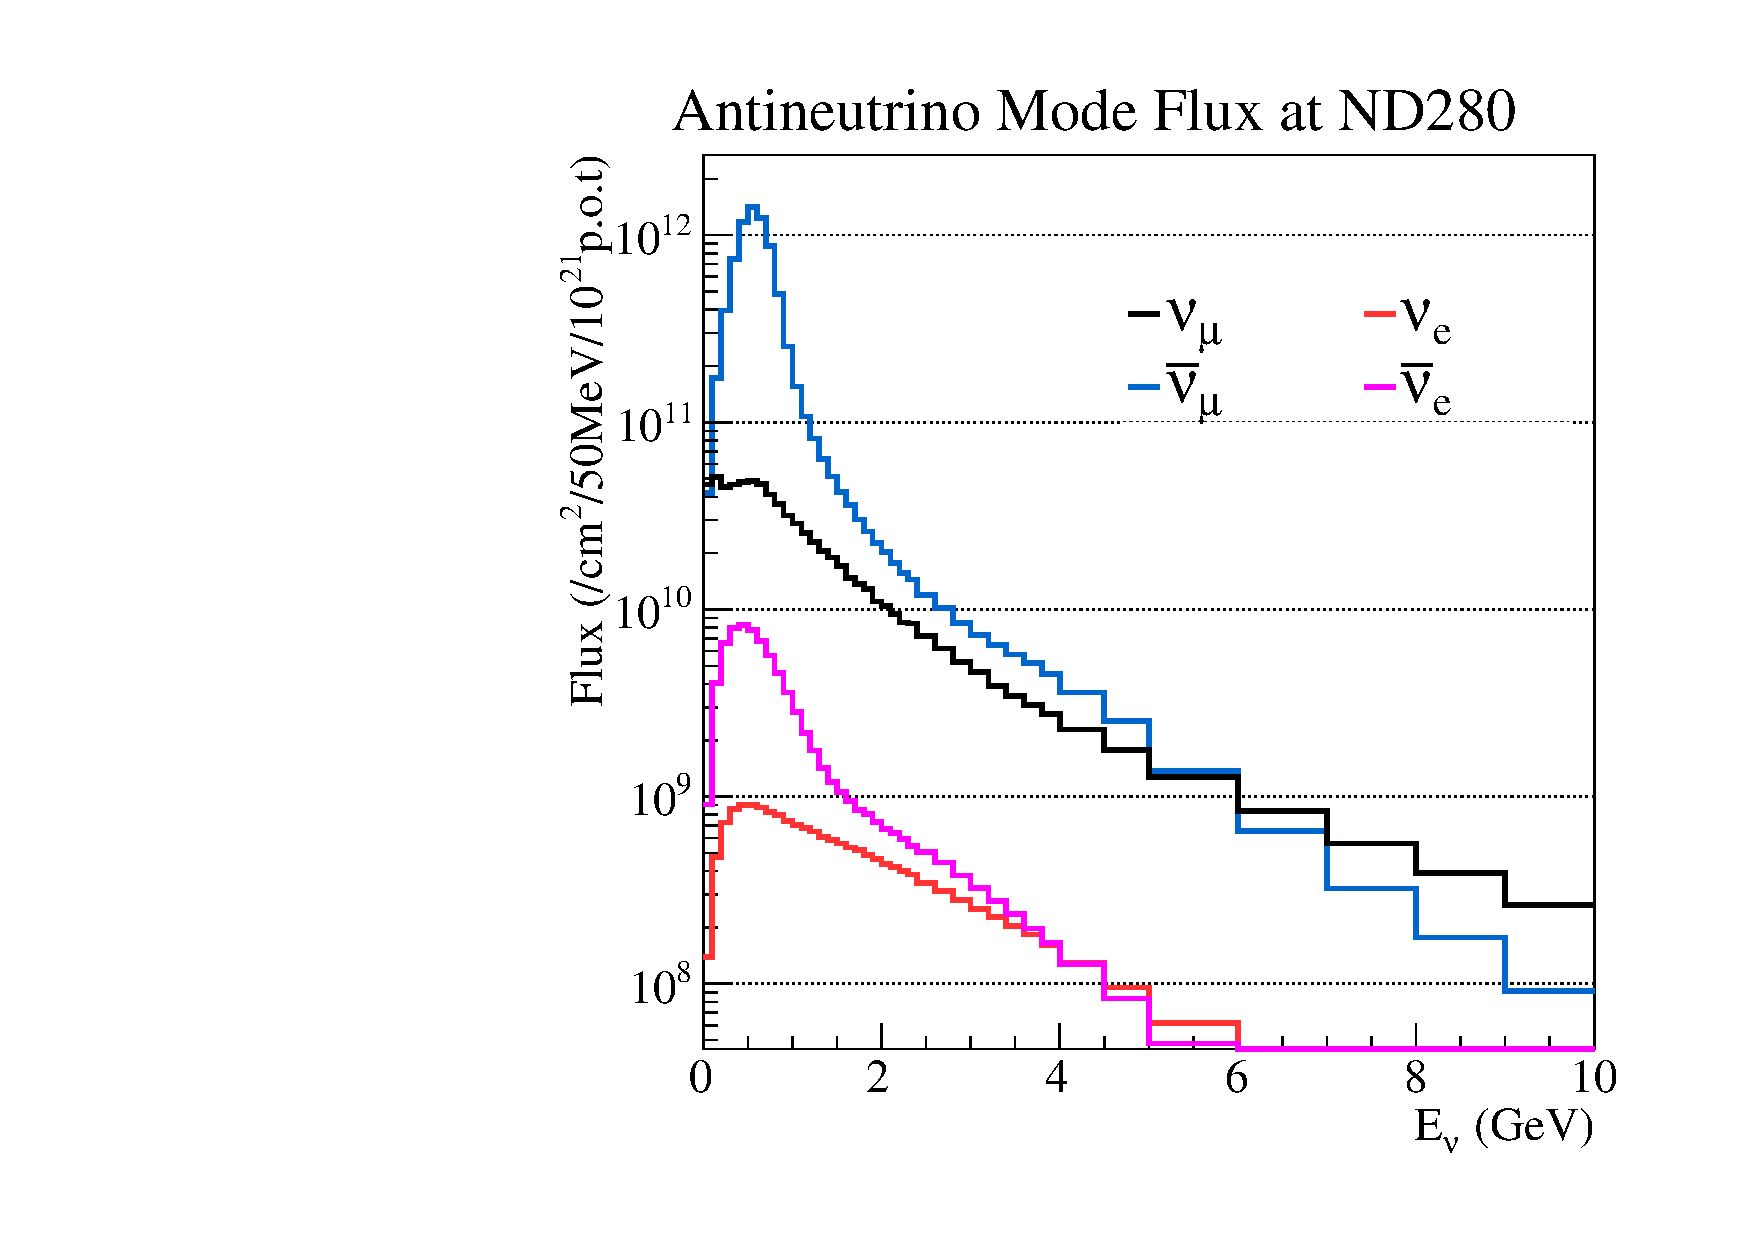
\includegraphics[width=\textwidth, trim={0mm 0mm 0mm 0mm}, clip,page=1]{figures/det_chap/beam/nd5_alltunedflux_run5c-7b_zoomed_antinu_13a}
		\caption{RHC}
	\end{subfigure}
	\caption{Simulated neutrino fluxes at ND280 in FHC and RHC modes}
	\label{fig:flux_1to8}
\end{figure}

\section{The Interactive Neutrino GRID}
\label{sec:ingrid}
Using the off-axis technique introduces the need for precise determination of the neutrino beam direction, as a 1 mrad uncertainty on the beam direction is followed by a 2-3\% uncertainty on the neutrino energy scale\cite{t2k_det}. Furthermore, sudden discontinuities of the beam or any of its subcomponents (e.g. magnetic horns or target) directly affect the neutrino flux, so measurements of the beam direction are made on a spill-by-spill basis.

The Interactive Neutrino GRID (INGRID) detector sits on-axis, 280 m downstream of the production target. It was designed to measure the neutrino beam profile to accurately predict the off-axis angle of ND280 and SK, and make inclusive neutrino cross-section measurements\cite{t2k_ingrid_xsec}. It has a cross shaped geometry and extends 10 m vertically and horizontally, shown in \autoref{fig:ingrid_det}. The cross consists of 14 identical modules and two off-axis detectors which measure the asymmetry of the neutrino beam. Each INGRID module has nine iron plates and 11 tracking scintillator plates, which are surrounded by veto planes on all sides to reject cosmic background\cite{t2k_ingrid}. Each module has a fiducial mass of iron at 7.1 tonnes, and the total cross spans roughly $1\sigma$ of the expected beam profile.
\begin{figure}[h]
	\begin{subfigure}[t]{0.47\textwidth}
		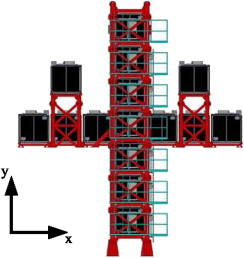
\includegraphics[width=\textwidth, trim={0mm 0mm 0mm 0mm}, clip,page=1]{figures/det_chap/ingrid/ingrid}
		\caption{Beam-view of INGRID}
	\end{subfigure}	
	\begin{subfigure}[t]{0.47\textwidth}
		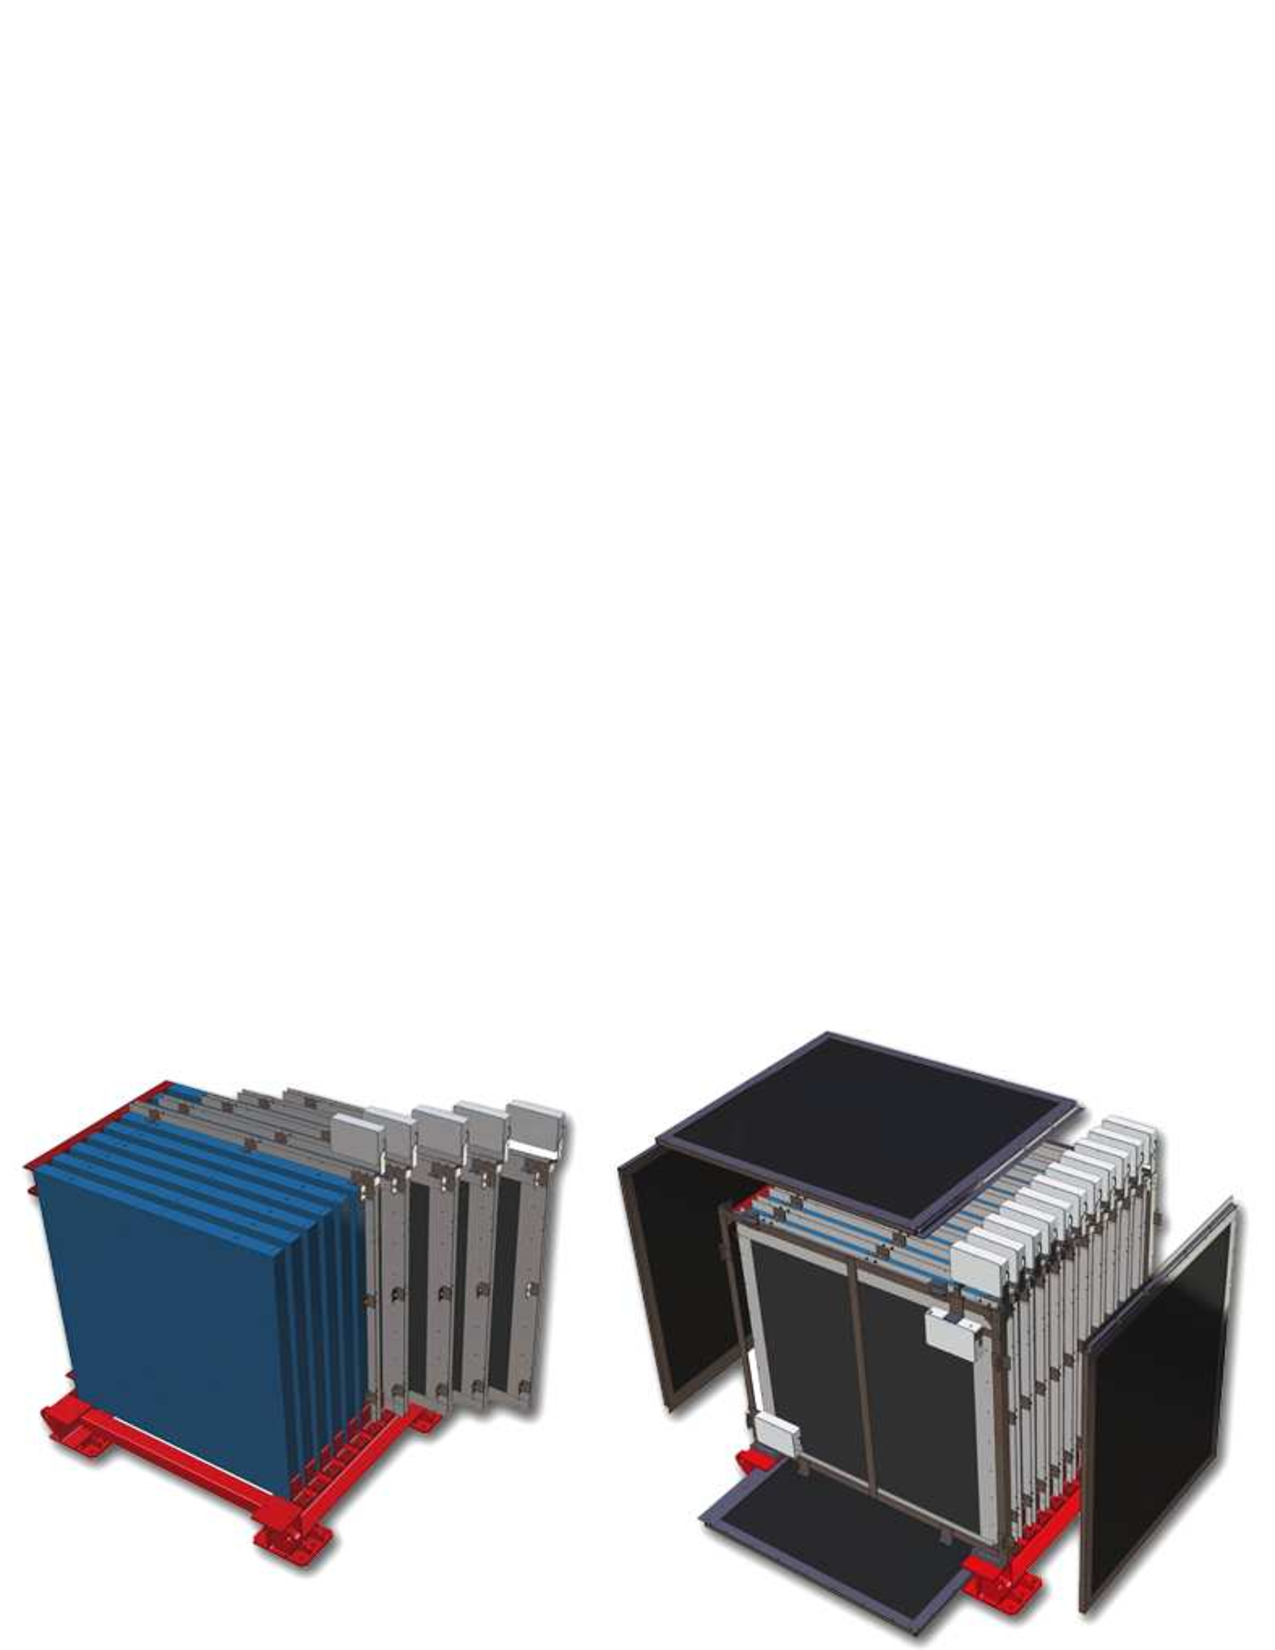
\includegraphics[width=\textwidth, trim={0mm 0mm 0mm 50mm}, clip,page=1]{figures/det_chap/ingrid/ingrid_module}
		\caption{An INGRID module}
	\end{subfigure}
	\caption{The INGRID experiment}
	\label{fig:ingrid_det}
\end{figure}
INGRID also has a second type of module---the proton module---designed to measure neutrino interactions on plastic scintillator. It consists of 34 tracking plates, similar to those in the INGRID modules but with different dimensions, surrounded by the same veto planes\cite{t2k_ingrid_proton}.

INGRID has measured the neutrino event rates within 2\% of expected, with a precision on the directionality of 0.2 mrad, all in agreement with expectation\cite{t2k_2015}, giving the neutrino beam center within 5 cm. The historical event rate and beam direction from MUMON and INGRID over the full beam period used in this thesis can be seen in \autoref{fig:ingrid_monitoring}. Generally, INGRID and MUMON agree within 0.2 mrad in both vertical and horizontal directions, and the neutrino event rate agrees with expectation.
\begin{figure}[h]
	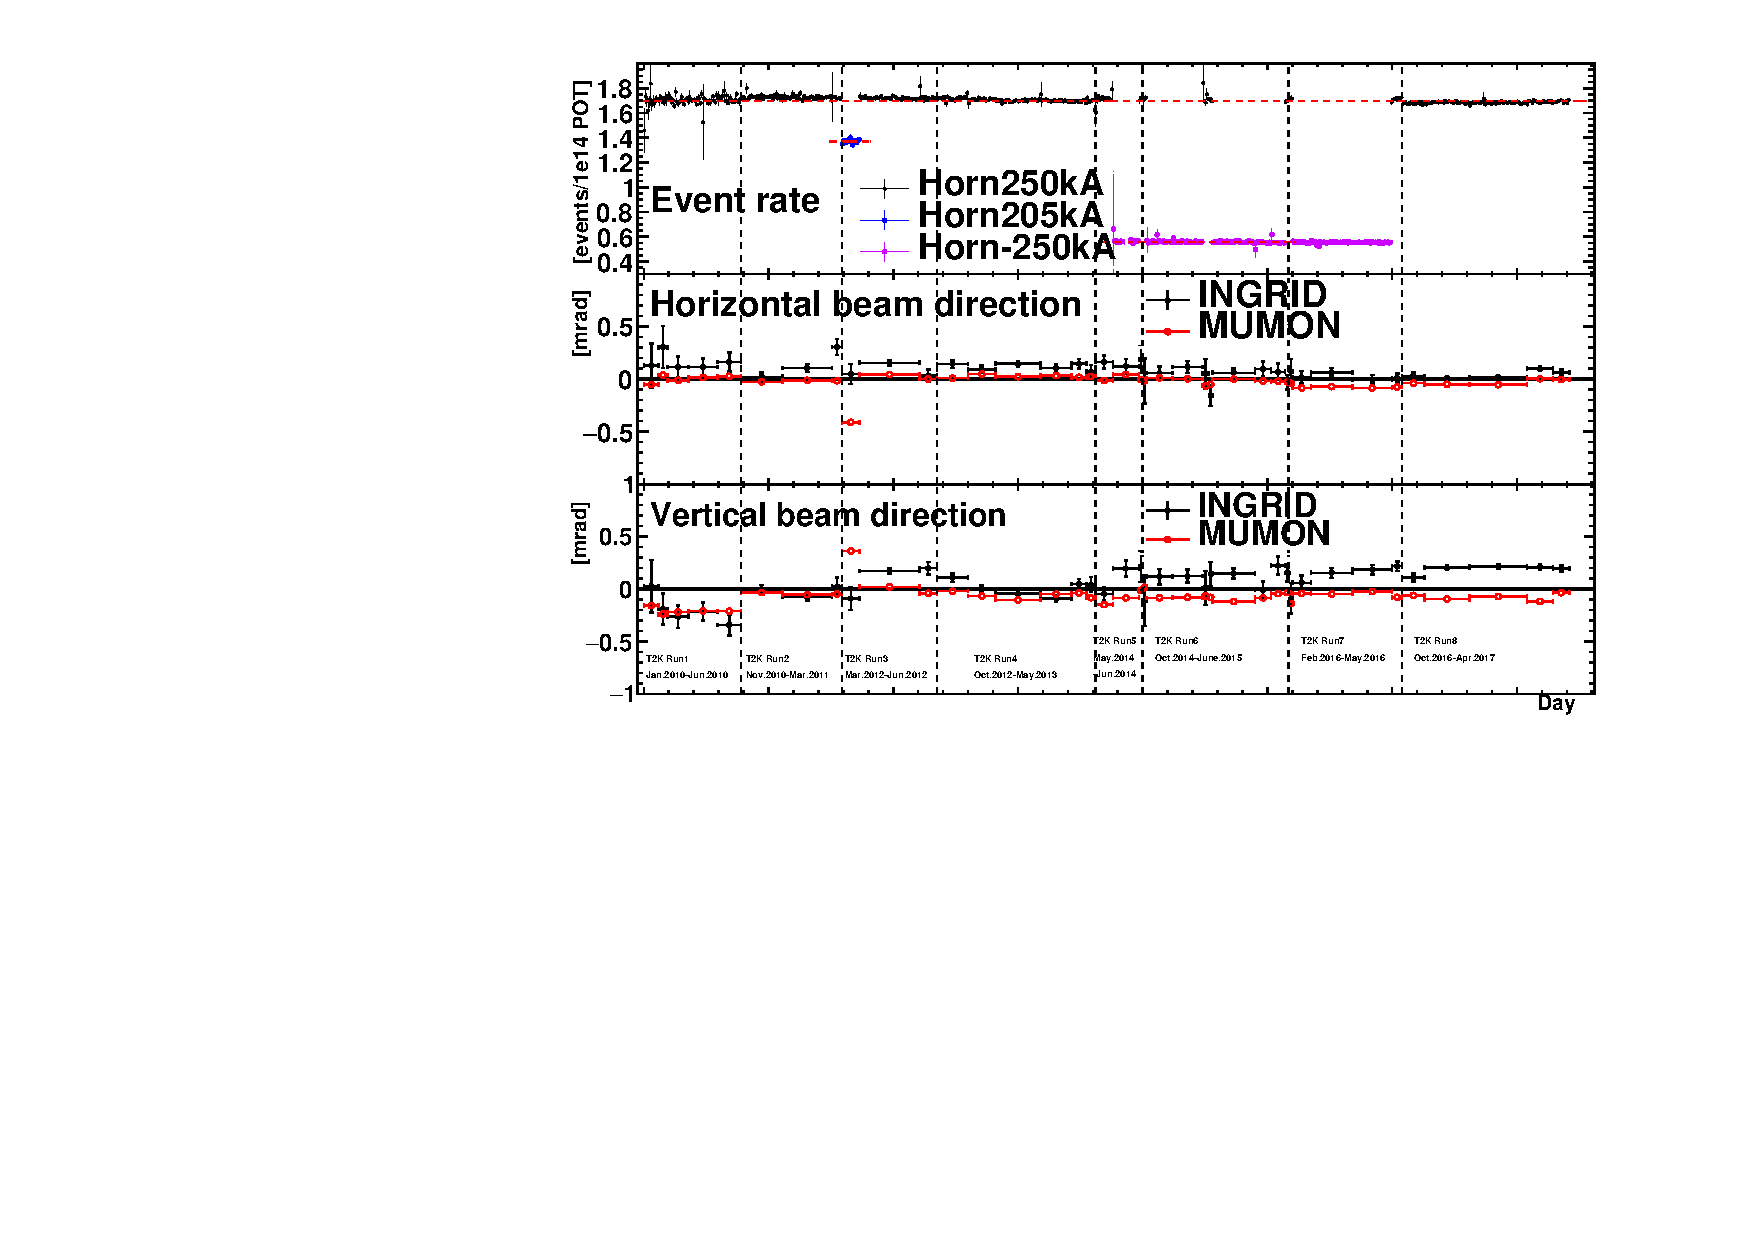
\includegraphics[width=0.8\textwidth, trim={0mm 0mm 0mm 0mm}, clip,page=1]{figures/det_chap/ingrid/INGRID_official_plot_until74}
	\caption{Beam characteristics measured by the INGRID and MUMON detectors over the T2K runs 1 through 8, used in this thesis.}
	\label{fig:ingrid_monitoring}
\end{figure}

\section{The Near Detector at 280 m}
\label{sec:nd280}
The off-axis near detector for T2K is called ND280, and its neutrino-nucleus interaction data is the subject of this thesis. In contrast to INGRID, ND280 was designed to accurately reconstruct and track particles emanating from a neutrino scattering vertex at its center.

ND280 surrounds its inner target sub-detectors, the two fine grained detectors (FGDs), by three time projection chambers (TPCs). This inner region is referred to as the ``tracker'' and it is enclosed by a lead-scintillator sampling electromagnetic calorimeter (ECal) on all but the upstream side, at which a dedicated $\pi^0$ detector, the P0D, is placed. The whole detector is bathed in a 0.2 T magnetic field to enable accurate sign selection and momentum measurements with the TPCs. The magnet yoke is in turn interleaved with a side muon range detector (SMRD) made of plastic scintillator strips which enable high angle tracking of $\mu$ and provides a cosmic tagger. The exploded detector view is shown in \autoref{fig:nd280_expl}.
\begin{figure}[h]
	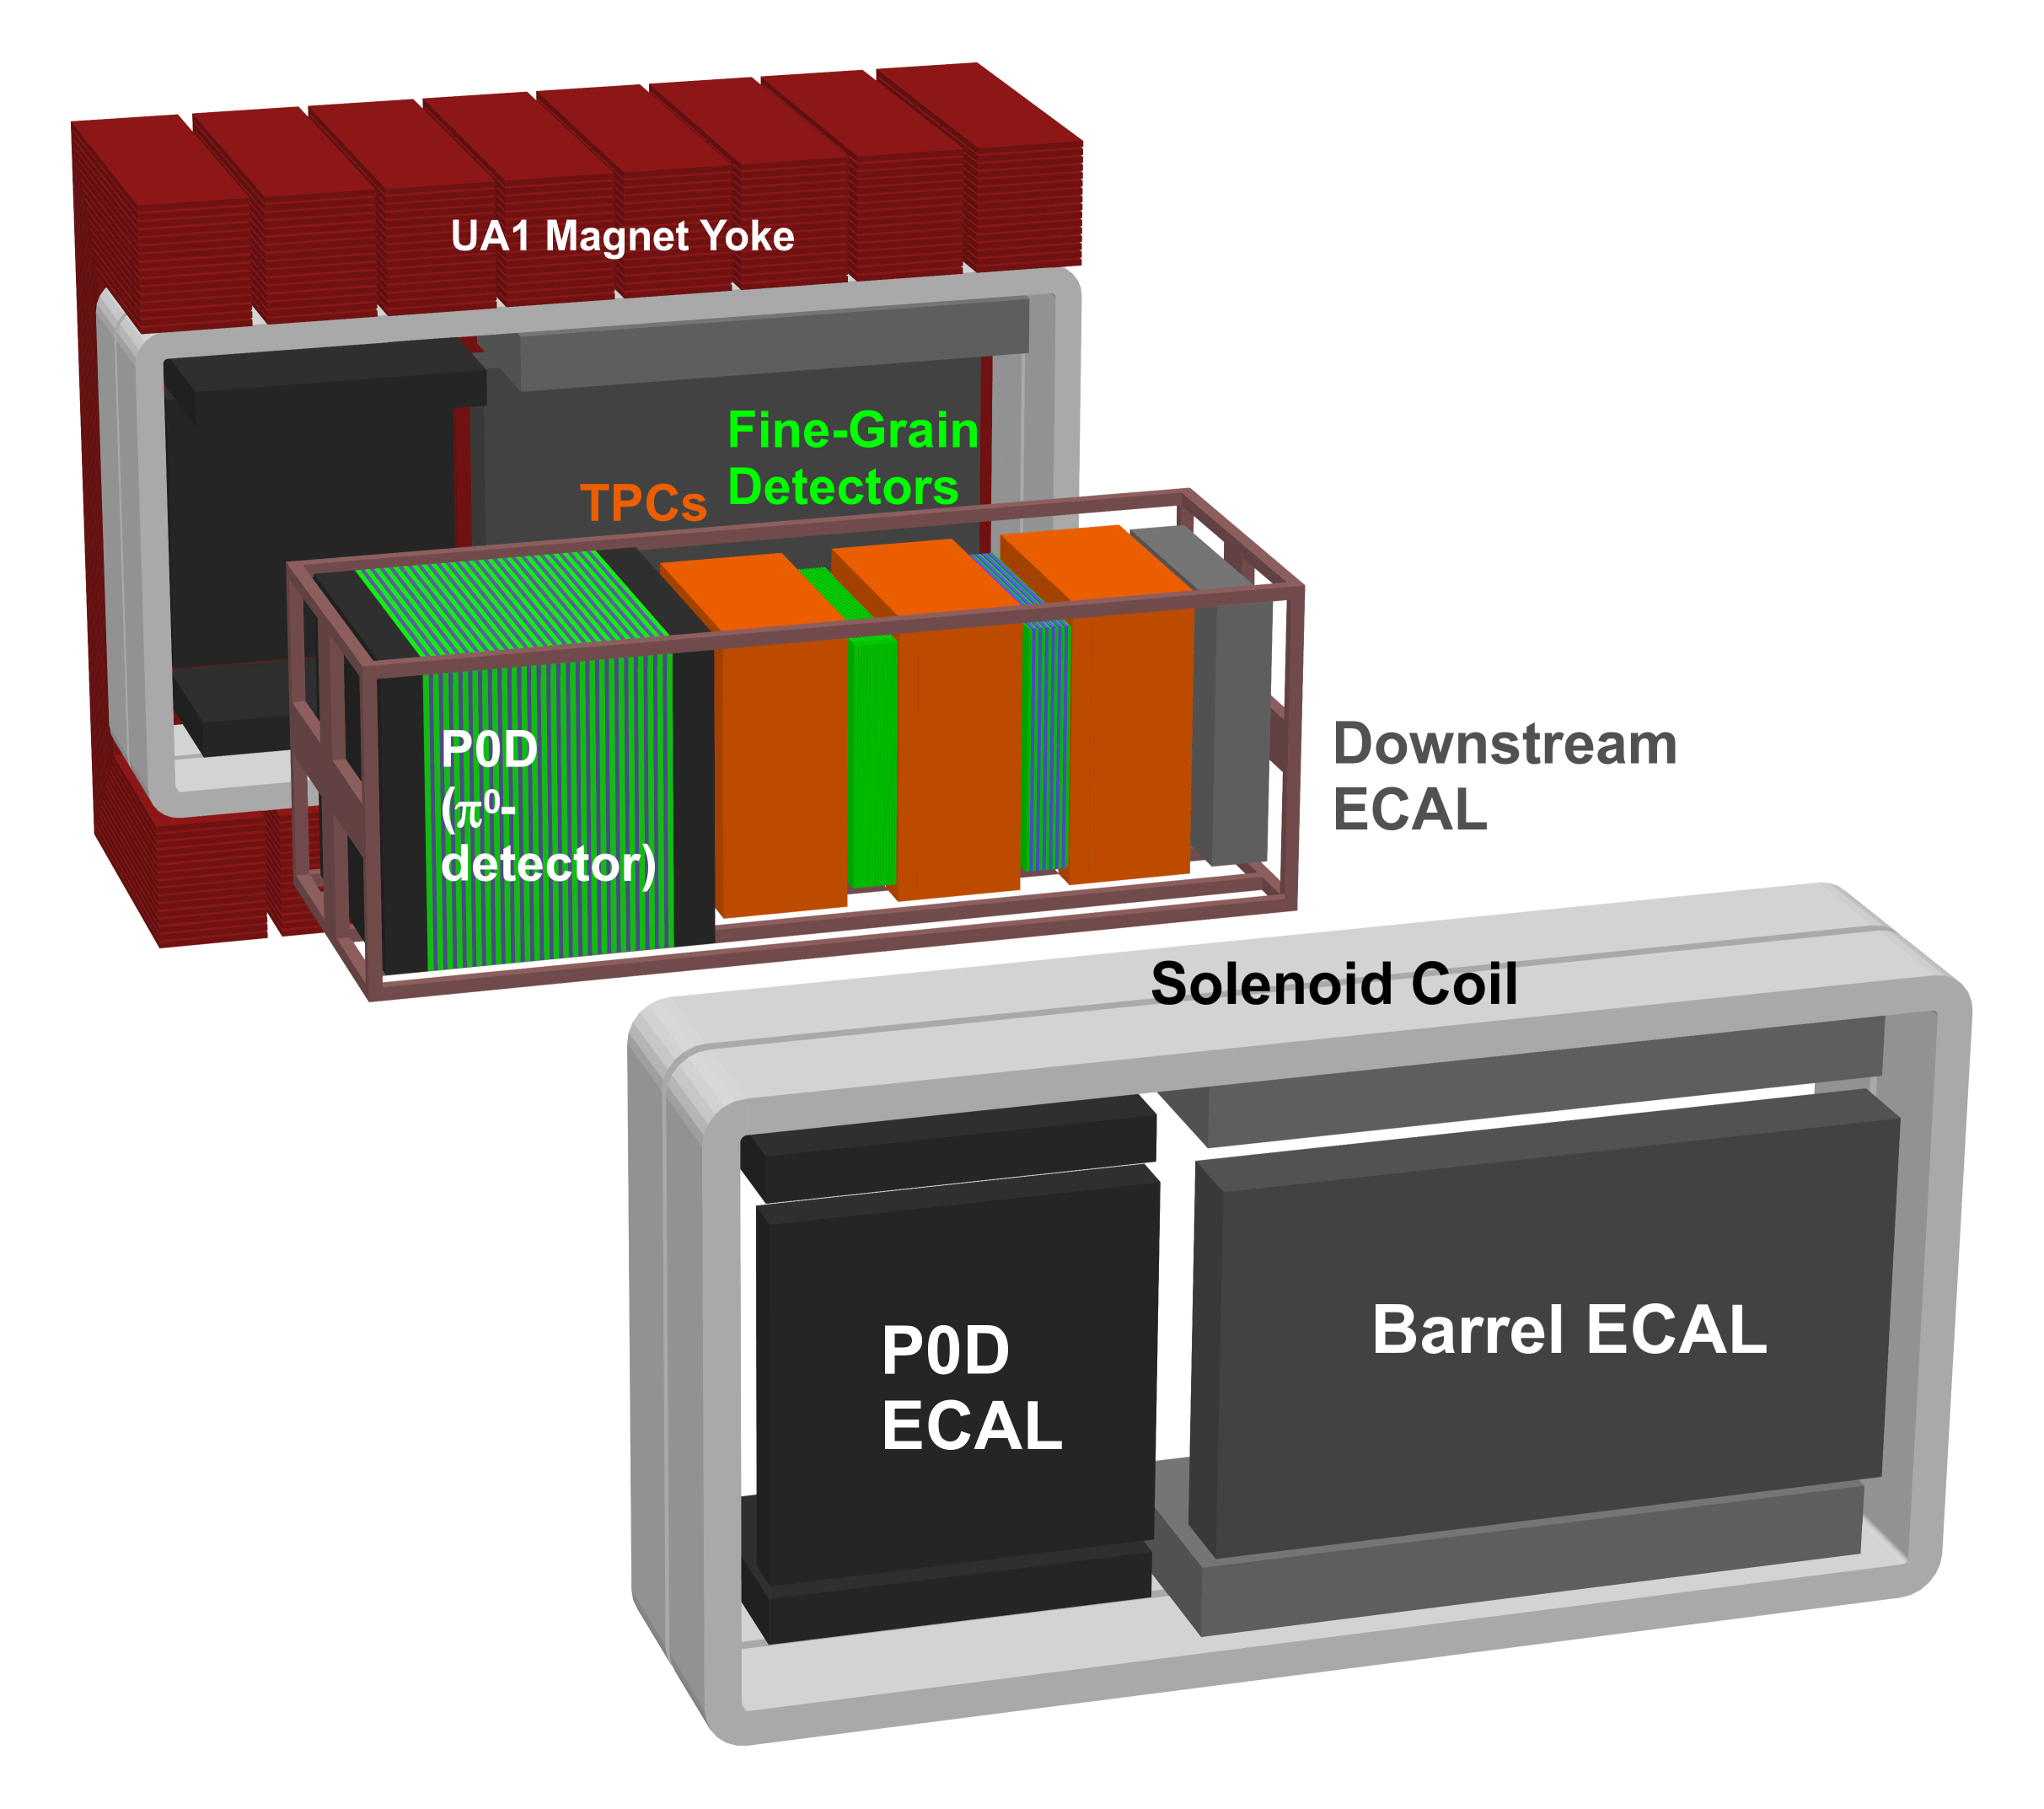
\includegraphics[width=0.6\textwidth, trim={0mm 0mm 0mm 0mm}, clip,page=1]{figures/det_chap/view/ND280Exploded-Text-Transparent-Large}
	\caption{The ND280 detector with its sub-detectors}
	\label{fig:nd280_expl}
\end{figure}

Since signal at SK is limited to the single ring $\mu$ and $e$ selections---vetoing any secondary rings from e.g. pions or high energy protons---the detector is designed around low multiplicity cross-section measurements. It also provides information on the single $\pi^0$ cross-sections, a major background for oscillation searches looking for $\nu_\mu \rightarrow \nu_e$.

The analyses presented in this thesis only use the FGDs and TPCs for particle detection and ID. Future analyses envisage using the ECal for high and backwards going selections and the P0D for forward-going events going through the first TPC.

\subsection{Fine Grained Detectors}
The two fine grained detectors (FGDs)\cite{t2k_fgd} are the central targets for ND280, providing measurements of flux, energy spectrum and electron neutrino contamination at the off-axis angle of SK ($2.5\deg$). Each FGD supply 1.1 tonnes of target material and extends $186.4\times186.4\times2.02\text{ cm}$ per scintillator plane. FGD1 sits most upstream of the two and is composed of 15 plastic scintillator XY planes, each plane having $2\times192$ bars. FGD2 provides a hybrid water-scintillator target, in which seven plastic scintillator XY planes identical to FGD1 are alternated with six 2.54 cm thick layers of water. The two FGDs thus measure interactions on both plastic CH---a common target in external neutrino scattering data---and $\text{H}_2\text{O}$---the target in SK.

The FGDs have the ability to reconstruct features of an event independent of the TPCs for contained particles. Isolated tracks are generally of lower momentum and deposit significant energy per unit track length. Summing the total deposited energy of an isolated FGD track provides a means to distinguish protons from minimally ionising particles. Furthermore, stopped pions may give rise to a delayed Michel $e$, which is searched for in the FGD reconstruction with an efficiency above 90\%\cite{thesis_christine}. Additionally, tracks with hits in the TPC are required to match FGD tracks to determine the interaction vertex. The FGD is also used to measure time-of-flight (ToF) of tracks to distinguish forward-going positive particles from backward-going negative particles, and vice versa, with a fast timing resolution of 3 ns.
\begin{figure}[h]
	\begin{subfigure}[t]{0.47\textwidth}
		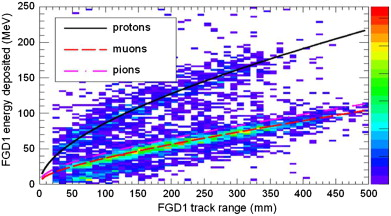
\includegraphics[width=\textwidth, trim={0mm 0mm 0mm 0mm}, clip,page=1]{figures/det_chap/fgd/fgd_byrange}
		\caption{Track-length and particle}
	\end{subfigure}
	\begin{subfigure}[t]{0.47\textwidth}
		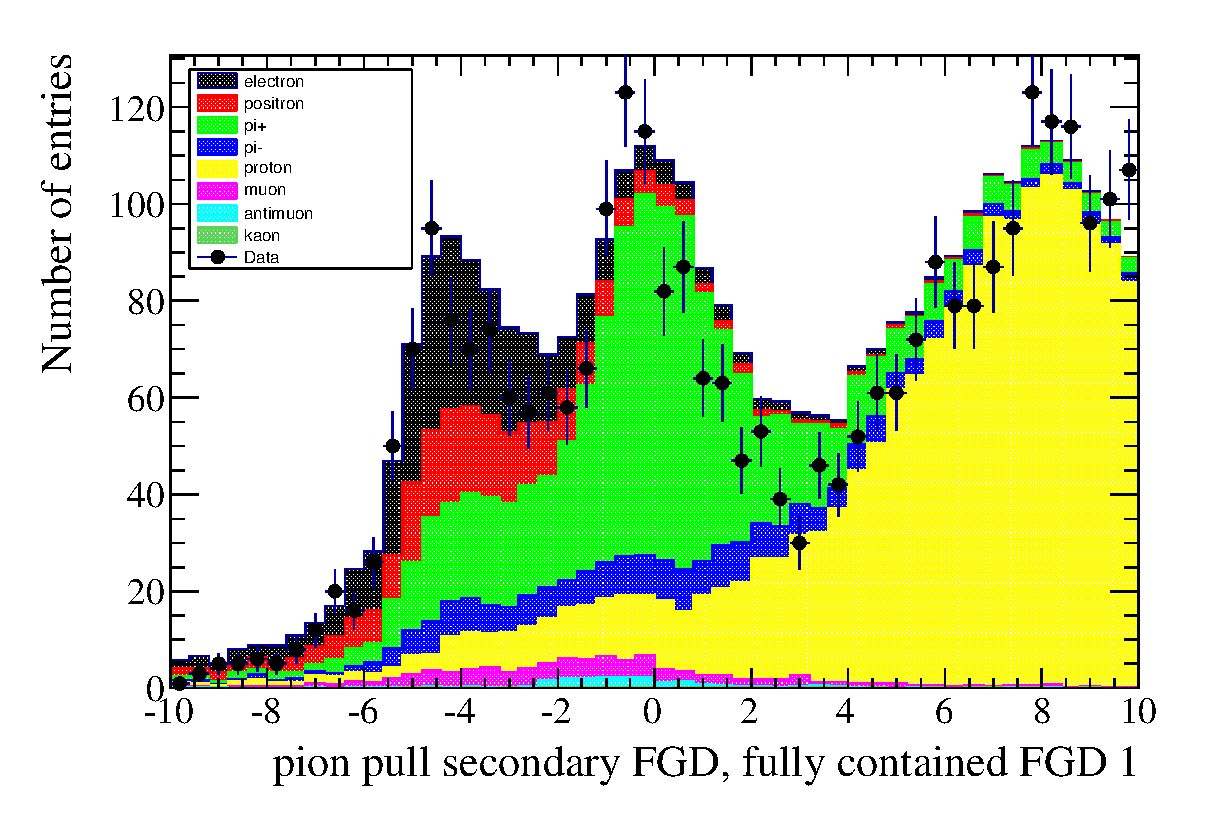
\includegraphics[width=\textwidth, trim={0mm 0mm 0mm 0mm}, clip,page=1]{figures/numu/Cuts/pull_secondarytrack_FGD_all_fullycontained}
		\caption{Particle pulls}
	\end{subfigure}	
	\caption{Parts of the FGD particle identification, using energy deposited with track length}
	\label{fig:fgd_reco}
\end{figure}

The measured track length and particle pulls for the pion hypothesis are shown in \autoref{fig:fgd_reco}. The three dominant distributions (electron/positron, pion and proton) are well separated in the pulls, agreeing relatively well with data.

The FGD is used for daily checks of the neutrino event rates and vertex distributions. It also acts as a cosmic trigger for stopping muons, whose selection is used to determine Michel $e$ efficiencies.

\subsection{Time Projection Chambers}
The three time projection chambers (TPCs)\cite{t2k_tpc} provide the majority of the tracking, energy loss, particle identification and momentum measurements in the ND280 detector. Each TPC is composed of an inner and an outer ``box''. The inner provides the field cage and the outer the ground potential. The inner box measures $1808\times2230\times850\text{ mm}$ and the outer box measures $2302\times2400\times974\text{ mm}$.  All TPCs use an $\text{Ar}:\text{CF}_4$:$\text{C}_4\text{H}_{10}$ mixture at 95:3:2, which ionises when charged particles pass through. The ionisation electrons are drifted toward bulk micromegas detectors\cite{micromegas_1, micromegas_2}, amplifying the charge. The maximum drift distance from central cathode to micromegas is 897 mm, and with the nominal cathode voltage at $-25\text{ kV}$ and micromegas at $-350\text{ kV}$, the drift field is $\sim 275\text{ V/cm}$. \autoref{fig:tpc_sys} provides a schematic of the TPC design.
\begin{figure}[h]
	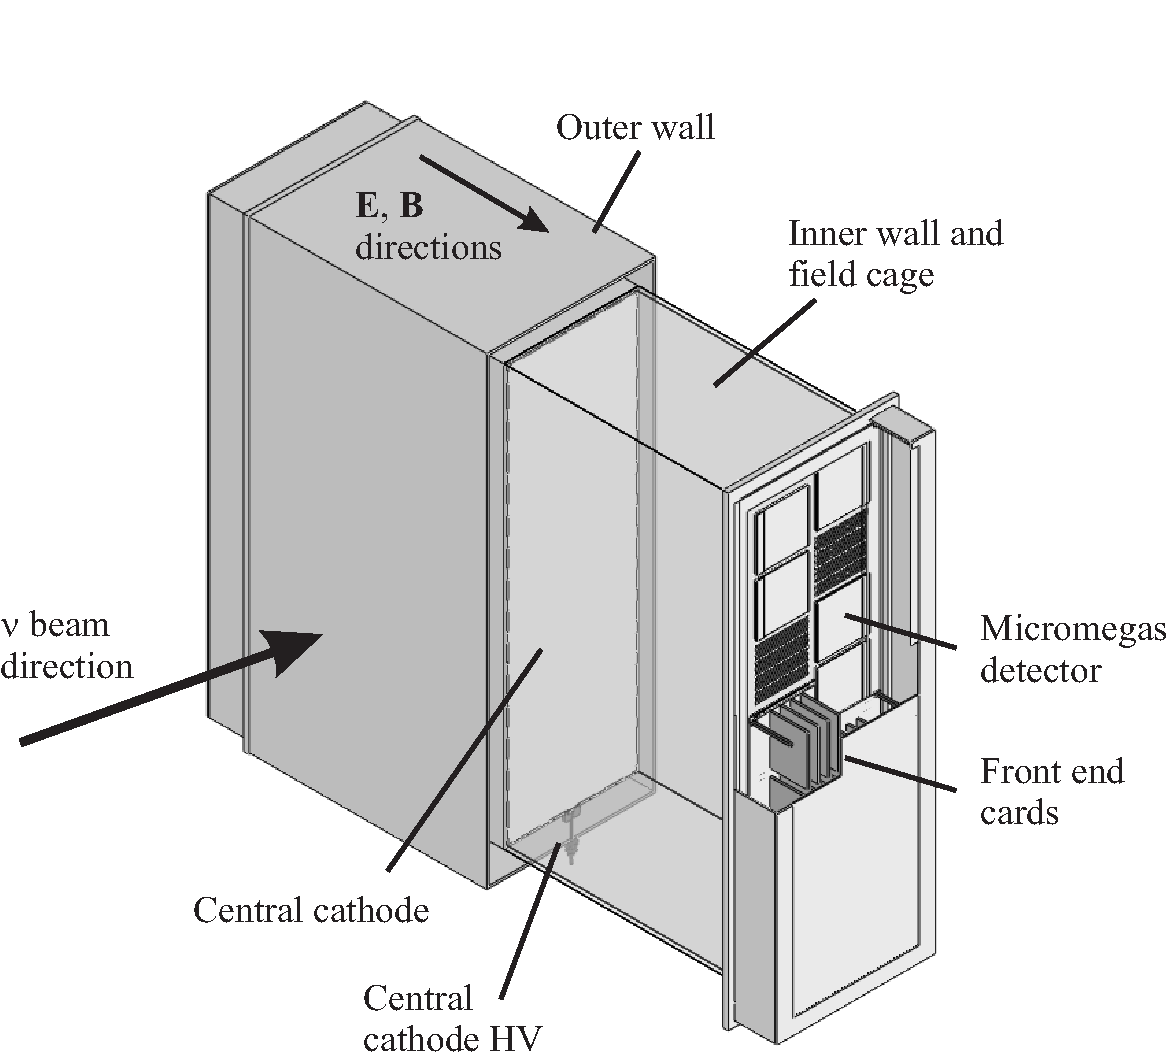
\includegraphics[width=0.4\textwidth, trim={0mm 0mm 0mm 0mm}, clip,page=1]{figures/det_chap/tpc/tpc_1}
	\caption{The ND280 TPC design, figure from \cite{t2k_tpc}.}
	\label{fig:tpc_sys}
\end{figure}

The bending of tracks in the magnetic field determines the momentum, and the readout provides a 3D image of the paths of traversing charged particles. Since two TPCs surround each FGD, they provide good tracking and multiplicity measurements of backward and forwards-going tracks. Furthermore, neutrino interaction cross-sections are generally highest for forward-going muons and pions, and a track traversing multiple TPCs gives an improved reconstruction.

The energy loss as a function of momentum in one TPC is shown in \autoref{fig:tpc_reco} for negatively and positively charged particles. Muon/electron distinction is achieved, and MIP resolution is $7.8\pm0.2\%$. Using the particle hypotheses outlined later in \autoref{sec:numu_sel}, the probability of assigning a muon to an electron hypothesis is 0.2\% for tracks below 1 GeV/c\cite{thesis_tpc}. There is also excellent ability to identify proton tracks with $p < 0.8 \text{ GeV}$.
\begin{figure}[h]
	\begin{subfigure}[t]{0.47\textwidth}
		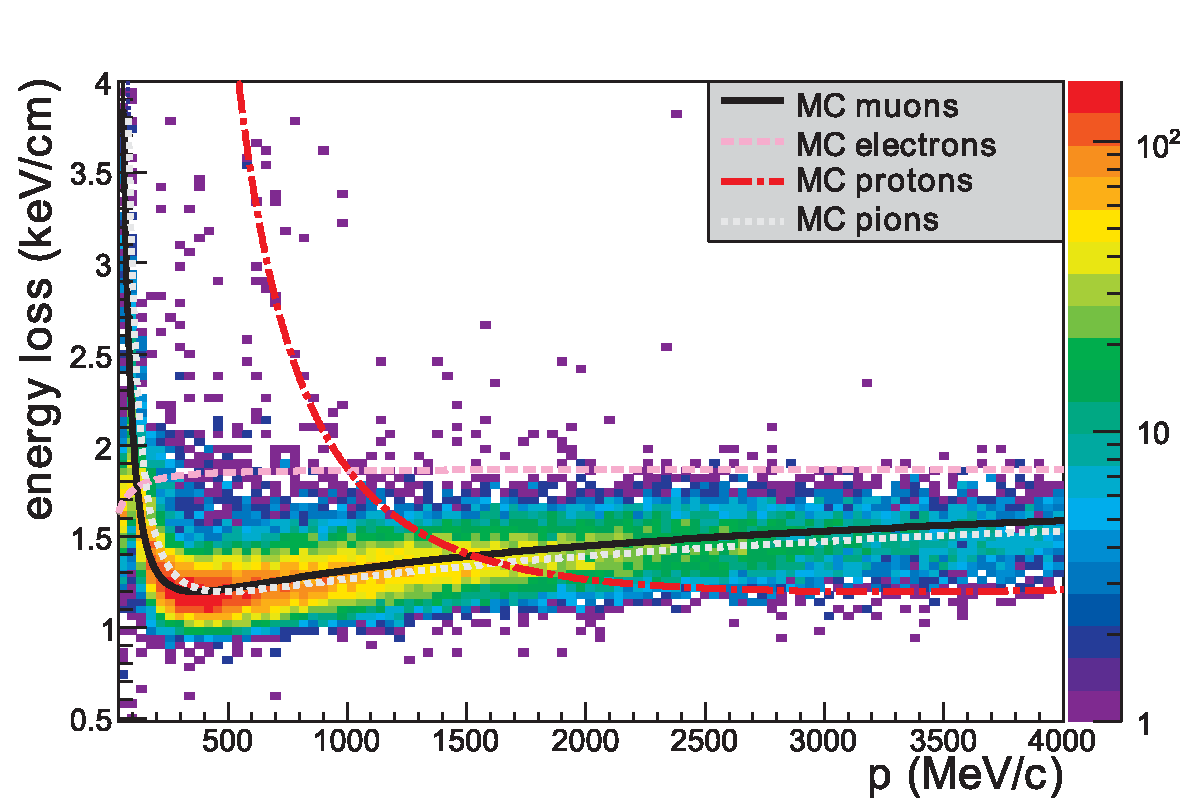
\includegraphics[width=\textwidth, trim={0mm 0mm 0mm 0mm}, clip,page=1]{figures/numu/TPC_PID_neg}
		\caption{Negative particles}
	\end{subfigure}
	\begin{subfigure}[t]{0.47\textwidth}
		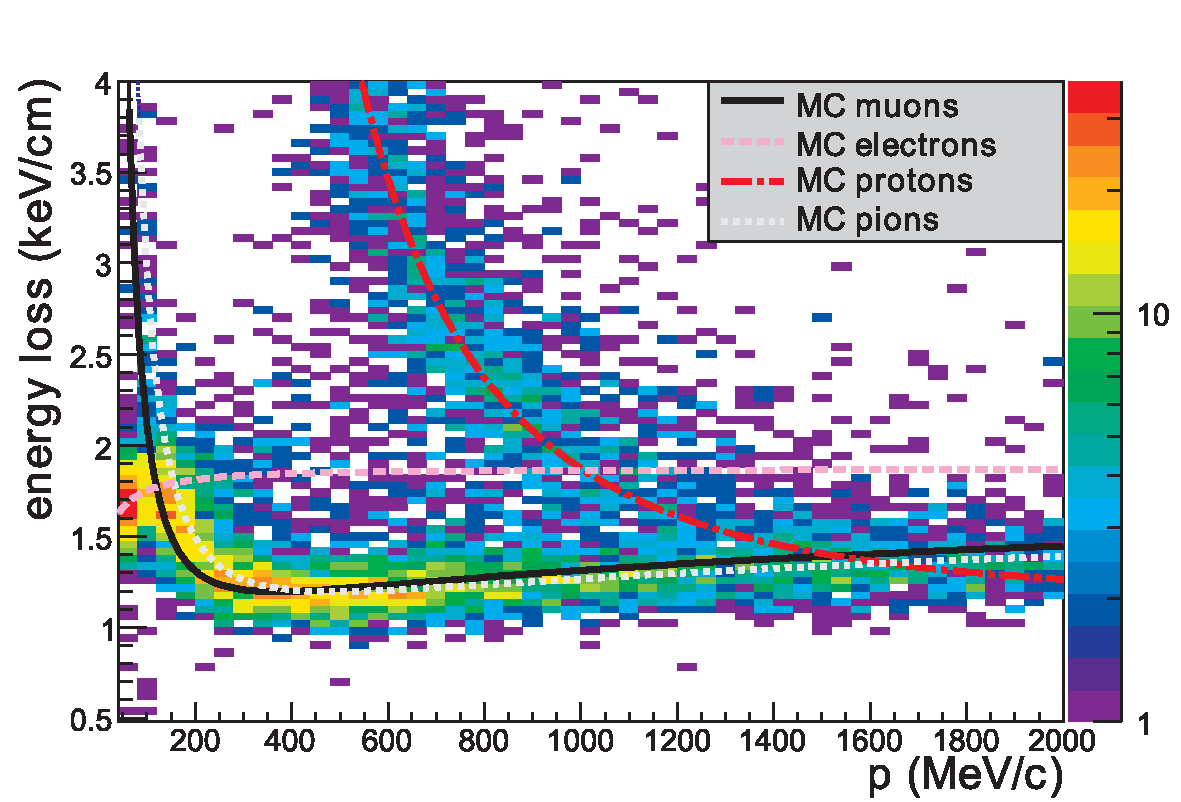
\includegraphics[width=\textwidth, trim={0mm 0mm 0mm 0mm}, clip,page=1]{figures/numu/TPC_PID_pos}
		\caption{Positive particles}
	\end{subfigure}	
	\caption{The energy loss in the TPC as a function of reconstructed momentum}
	\label{fig:tpc_reco}
\end{figure}

\subsection{Electromagnetic Calorimeter}
The ND280 electromagnetic calorimeter (ECal)\cite{t2k_ecal} is designed to complement the tracker in full event reconstruction due to its near hermetic coverage of the tracker and P0D regions. It measures photon showers' energy and directions, and is used to distinguish electrons from muons from pions by shower shape. Its primary purpose is to tag and reconstruct $\pi^0$s from the tracker.

The ECal has three main sections: 1) the barrel ECal, surrounding the inner tracking detectors, 2) the downstream ECal, sitting after the last TPC, and 3) the P0D Ecal. The tracker (barrel+downstream) ECal was designed as a tracking calorimeter and reconstructs electromagnetic showers, complementing the TPC where high-angle particles may leave few hits. The P0D-ECal was designed to tag escaping energy and perform photon/muon separation, since the P0D performs its own shower reconstruction. The ECals are all made of scintillating polystyrene bars $40\times10\text{ mm}$ which are adhered to $1.75\text{ mm}$ lead sheets. The ECal design was based on good detection efficiency of $\pi^0$s emanating from the tracker region. The barrel-ECal has 31 layers and the downstream has 34 layers, corresponding to 10 and 11 electron radiation lengths, required to ensure $\sim50\%$ of the energy from photo showers from a $\pi^0$ decays is contained. The P0D-ECal has six scintillator layers with 4 mm thick lead sheets.

The downstream ECal is $2300\times2300\times500\text{ mm}$ with 50 $2000\text{ mm}$ long scintillator bars. The four barrel ECal top and bottom modules are $4140\times1676\times462\text{ mm}$ and the two side barrel ECals are $4140\times2500\times462\text{ mm}$. The top and bottom ECals have $1520\text{ mm}$ bars, and the side have $2280\text{ mm}$ bars, perpendicular to the beam direction, and 15 $3840\text{ mm}$ bars parallel to the beam. The P0D ECal is 155 mm deep, with the top and bottom modules being $1584\text{ mm}$ wide and the sides being $2898\text{ mm}$ wide, with $2454\text{ mm}$ length.

\subsection{Pi-zero Detector}
The pi-zero detector (P0D)\cite{t2k_p0d} was designed to measure the NC1$\pi^0$ production cross-section, a large systematic for \nue appearance.

The design of the P0D is shown in \autoref{fig:nd280_p0d}. The central water target, consisting of 13 alternating scintillator-water bags-brass sheet planes, is surrounded by an upstream and downstream ECal which is void of water and seven planes each. The entire P0D consists of 40 modules, each being two perpendicular arrays of triangular scintillator bars. Each vertical bar (134 per P0D module) is 2200 mm long, and the horizontal bars are 2340 mm long (126 per P0D module)\footnote{Originally designed for the MINER$\nu$A experiment\cite{minerva_design}}. The active target of the P0D is $2103\times2239\times2400\text{ mm}$ and the mass with (without) water is 16.1 (13.3) tonnes.
\begin{figure}[h]
	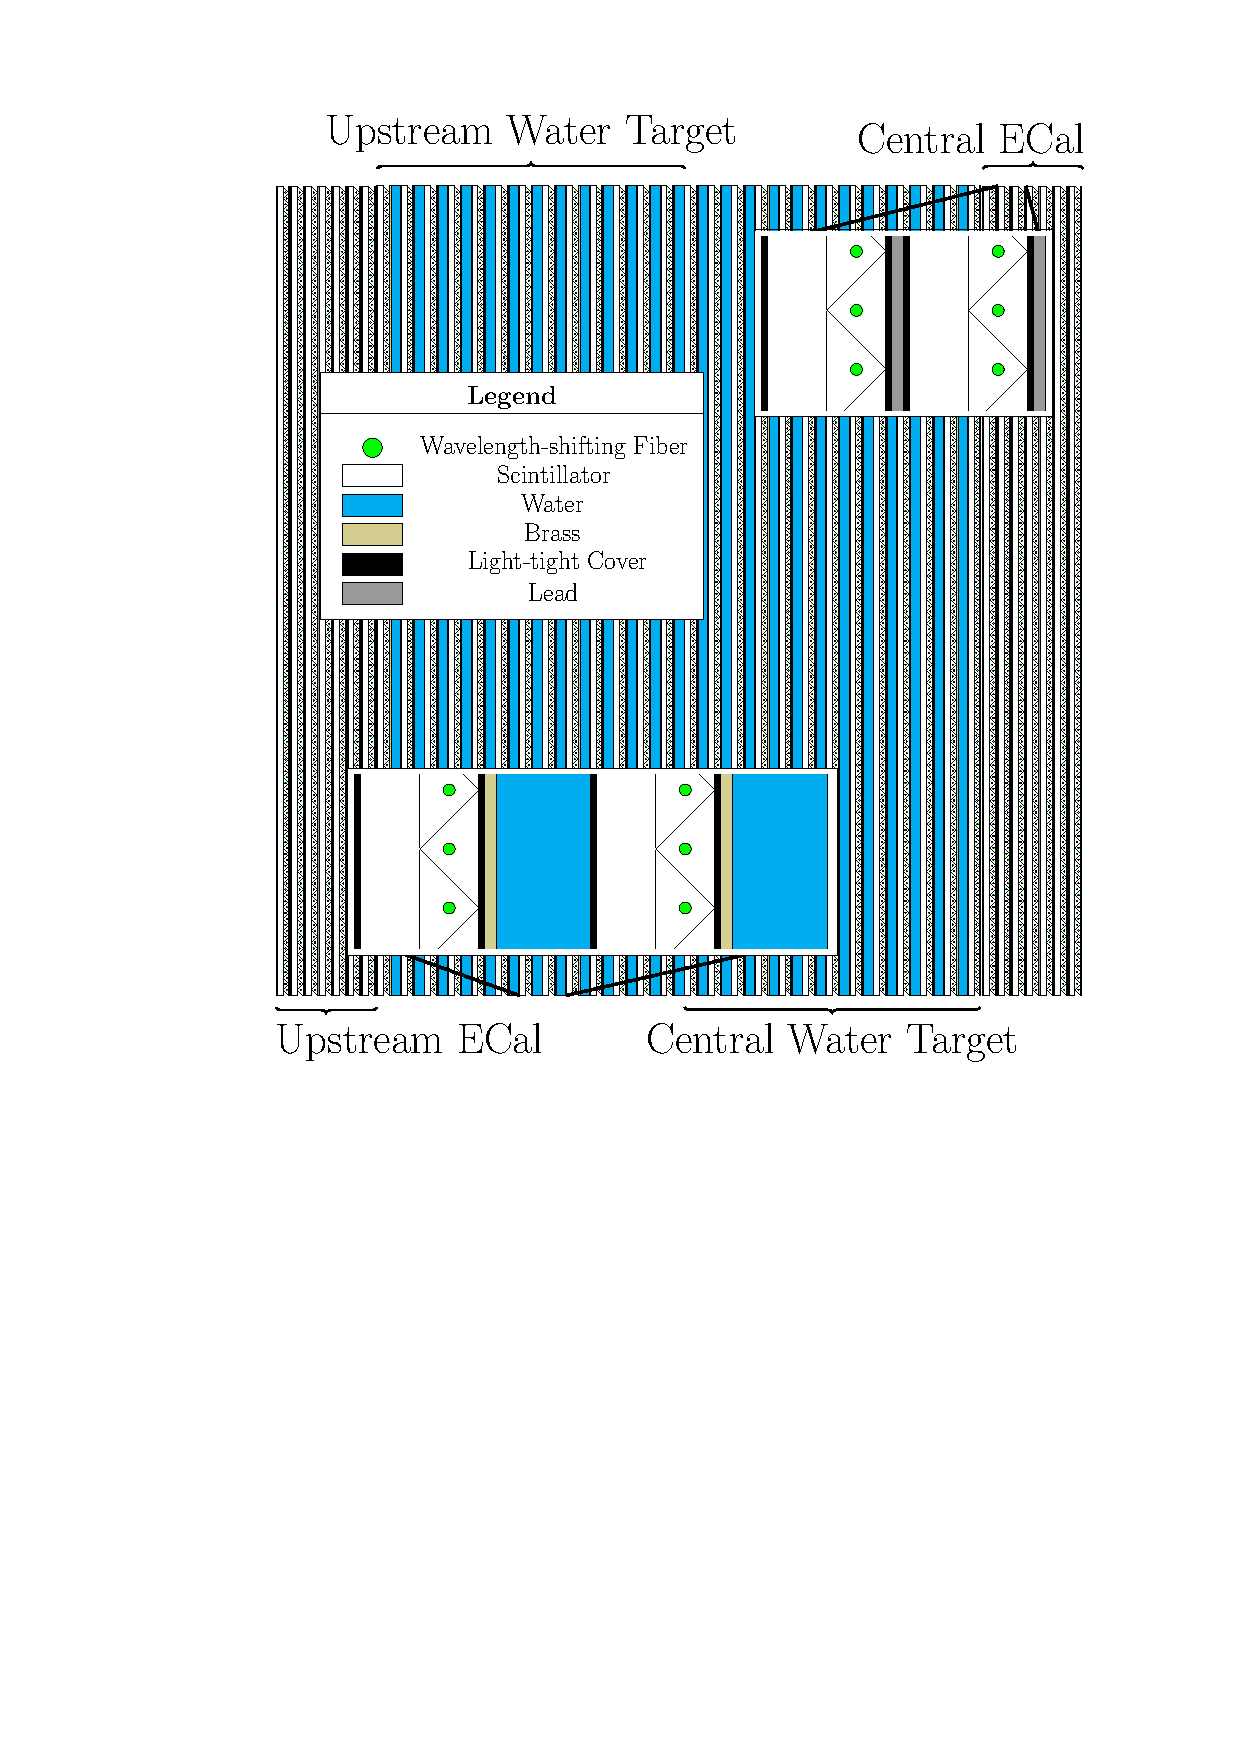
\includegraphics[width=0.6\textwidth, trim={0mm 110mm 0mm 0mm}, clip,page=1]{figures/det_chap/p0d/p0d.pdf}
	\caption{The ND280 P0D side-view}
	\label{fig:nd280_p0d}
\end{figure}

\subsection{The UA1/NOMAD Magnet and Side Muon Range Detectors}
The entirety of the above detector system (FGD+TPC+ECal+P0D) is placed inside the refurbished UA1/NOMAD dipole magnet. It is operated at 2.7 kA to produce a uniform horizontal magnetic field of 0.2 T. The  yoke is split into two sections, each made of eight C-shaped flux return yokes. The inner volume of the magnet is $7.0\times3.5\times3.6\text{ m}$, placing the main spatial limitations on ND280.

The side muon range detector (SMRD)\cite{t2k_smrd} sits in the innermost gaps of the UA1 magnet return yoke, surrounding the entire ECal, P0D and tracker. It was designed to measure muons which escape the tracker at high angles, punching through the FGD, ECal and SMRD but leaving few or no TPC hits. The momentum can be inferred from range in the iron and SMRD and the tracks can be reconstructed using FGD-ECal-SMRD matching with $\sim70\%$ efficiency. The SMRD additionally provides a cosmic trigger.
\begin{figure}[h]
	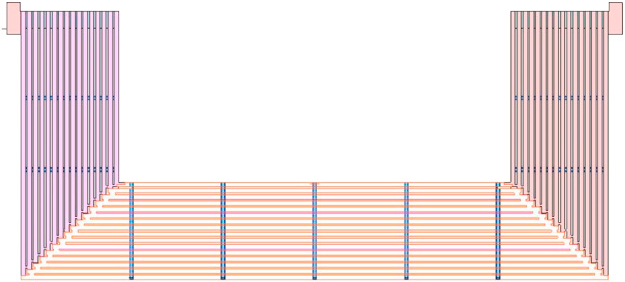
\includegraphics[width=0.4\textwidth, trim={0mm 0mm 0mm 0mm}, clip,page=1]{figures/det_chap/smrd/ua1_smrd}
	\caption{A section of the UA1 magnet yoke, side-view}
	\label{fig:nd280_ua1}
\end{figure}

Shown in \autoref{fig:nd280_ua1}, there are 16 iron plates in the magnet yoke, each 48mm thick and separated by 17 mm spacers, leaving space for 15 layers of scintillator. The SMRD consists of 192 horizontal and 248 vertical modules in total. The modules measure $9\times686\times955\text{ mm}$ and $9\times892\times955\text{ mm}$ for horizontal and vertical modules respectively. Each horizontal module has four scintillation counters $7\times167\times875\text{ mm}$ and vertical modules have five $7\times175\times875\text{ mm}$, totalling 768 horizontal and 1240 vertical counters. There are three layers of modules in the yoke on the upstream sides, and four layers for the 6th downstream yoke, with six layers for the two most downstream yokes.

\section{Super-Kamiokande}
\label{sec:sk}
The Super-Kamiokande (SK)\cite{t2k_sk, t2k_sk2, t2k_sk3} detector has served to measure proton decay, solar and atmospheric neutrino oscillations since 1996 with SK-I. Starting with K2K in 1999\cite{k2k_design}, Super-Kamiokande has also been serving as a far detector for long baseline accelerator neutrino oscillation searches, and continues to do so for T2K with SK-IV. The detector is placed 295 km from the production target in the Kamioka mine in Ikenoyama, located in Gifu, Japan. The mine provides roughly 1 km rock overburden---or 2.7 km equivalent water overburden---drastically reducing cosmogenic backgrounds. A sketch of the detector in the mine is shown in \autoref{fig:sk_schematic}.
\begin{figure}[h]
	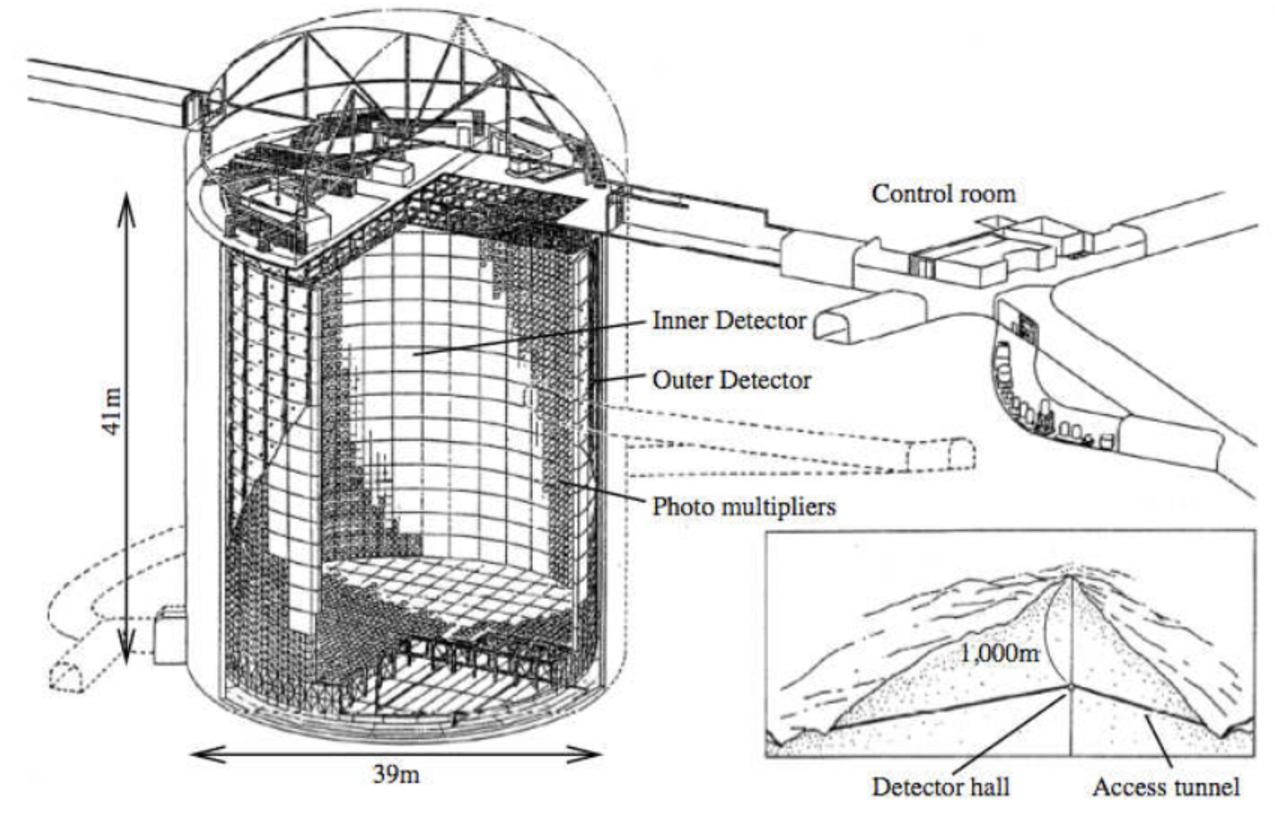
\includegraphics[width=0.6\textwidth, trim={0mm 0mm 0mm 0mm}, clip,page=1]{figures/det_chap/sk/sk.pdf}
	\caption{The Super-Kamiokande detector in Ikenoyama}
	\label{fig:sk_schematic}
\end{figure}

The detector consists of 50,000 (25,000 fiducial) tonnes of ultra-pure water in a $41.4\times39.3\text{ m}$ cylindrical tank. It is split into an inner (ID) and outer (OD) detector with inner dimension $36.2\times33.8\text{ m}$, where the OD surrounds the ID. The ID and OD are separated by a Tyvek and ``blacksheet'' barrier, and the ID has 11,146 inward-facing 20-inch PMTs, and the OD---providing a veto and shielding for the inner detector---has 1,885 8-inch PMTs facing outwards. The ID has approximately 40\% photo-coverage and provides excellent $\mu/e$ separation, crucial to differentiate muon neutrino disappearance from electron neutrino appearance.

Particle detection in SK happens primarily through production of Cherenkov light. The muon/electron separation occurs primarily by ring ``fuzziness'', indicating the amount of rescattering of the charged particle. Muons and pions are generally highly penetrating whereas electrons rescatter often and shower at T2K energies. The former produces sharp rings whereas electrons produce fuzzy rings. The number of delayed Michel $e$ is also used to identify contained muons and pions, and tracks with kinked trajectories are used to discern rescattered pions.
\begin{figure}[h]
	\begin{subfigure}[t]{0.48\textwidth}
		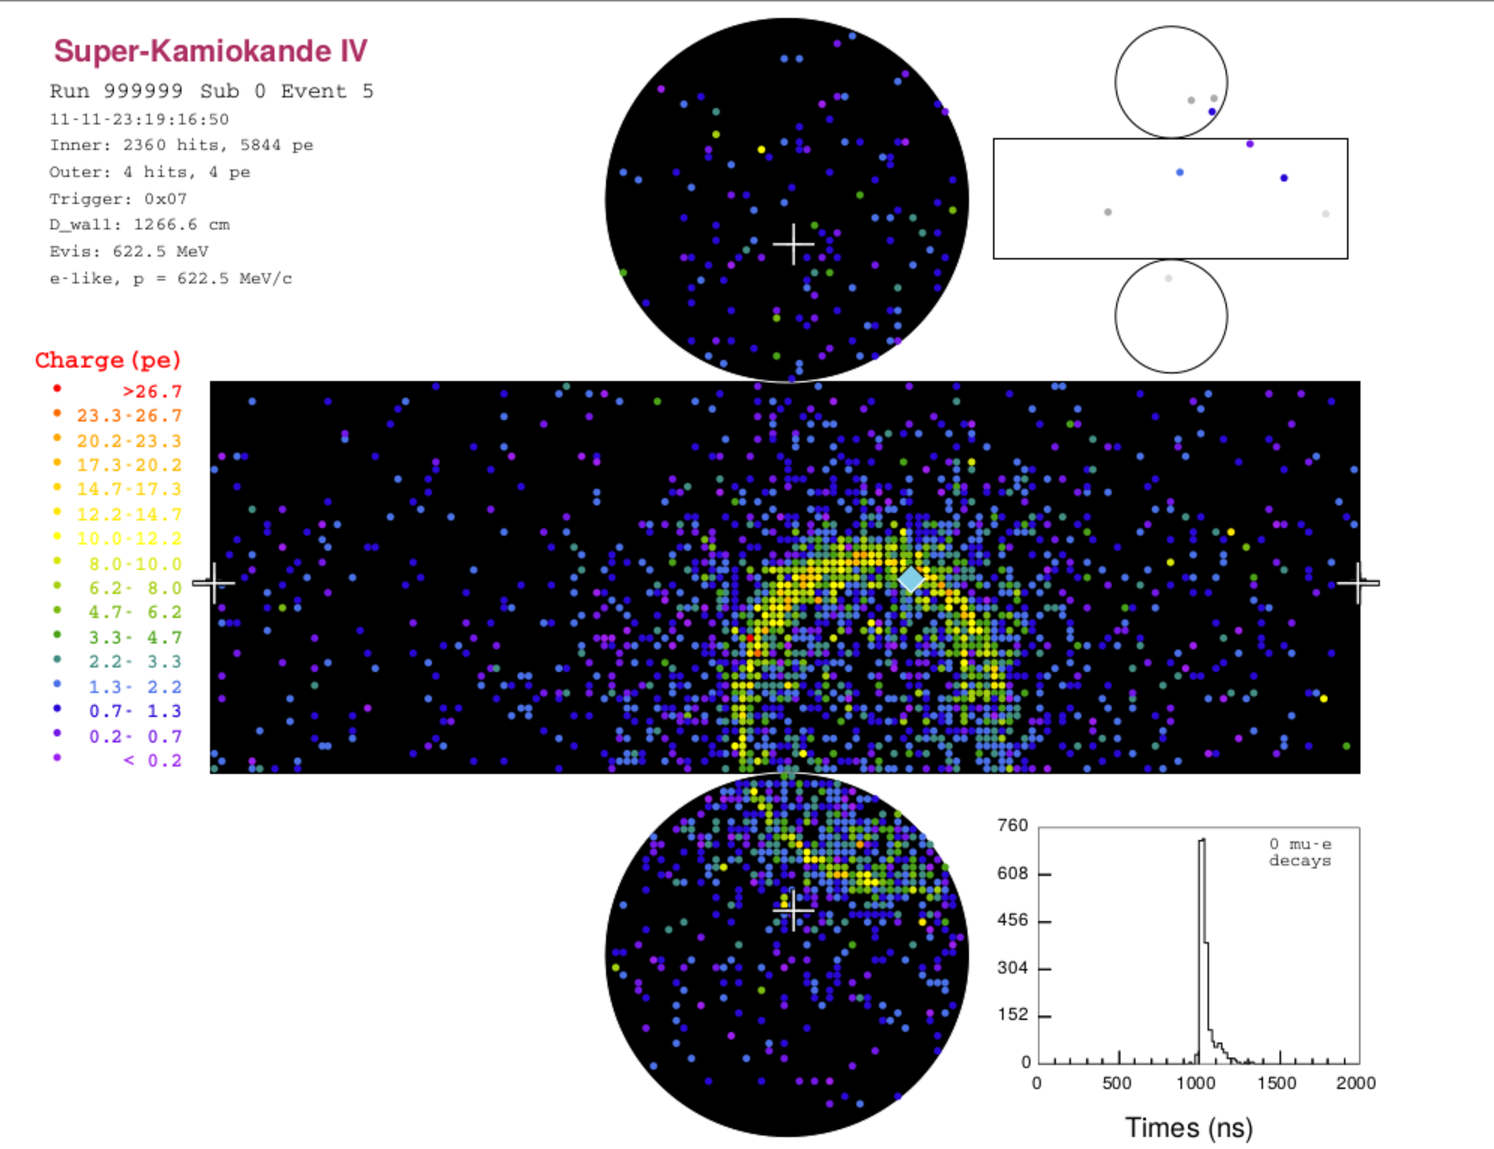
\includegraphics[width=\textwidth, trim={0mm 0mm 0mm 3mm}, clip,page=1]{figures/det_chap/sk/elike.pdf}
		\caption{$e$-like, $p=622.5\text{ MeV}$}
	\end{subfigure}
	\begin{subfigure}[t]{0.48\textwidth}
		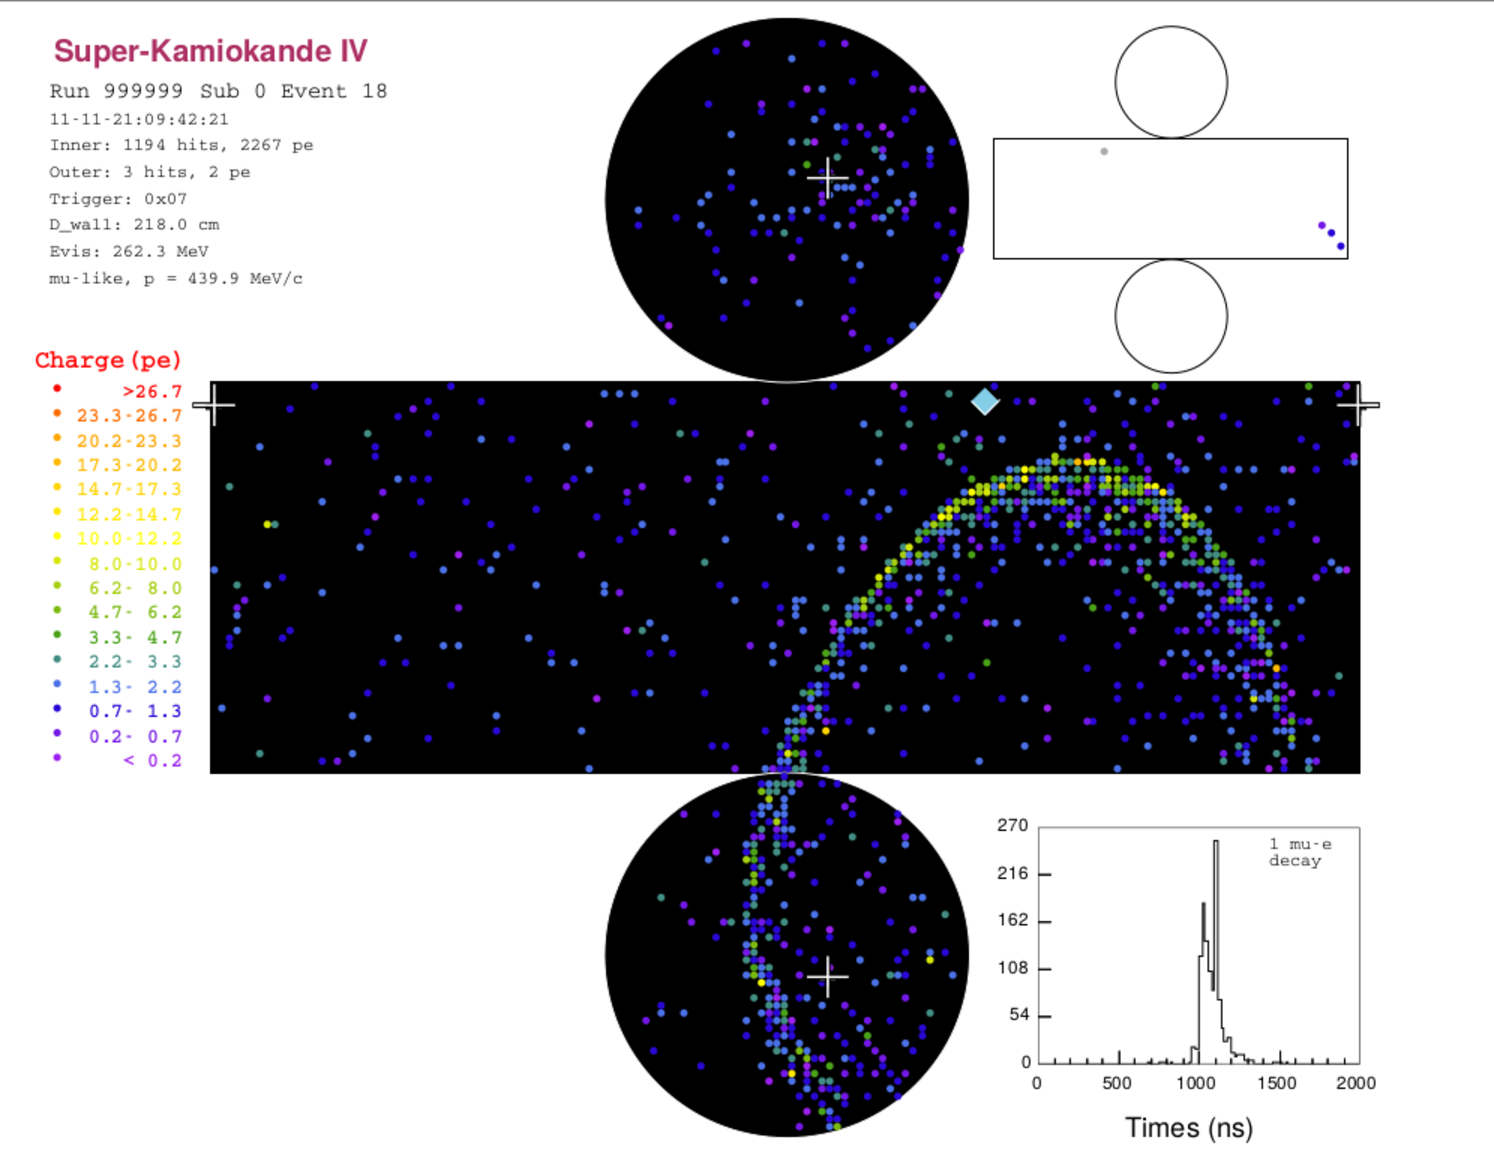
\includegraphics[width=\textwidth, trim={0mm 0mm 0mm 3mm}, clip,page=1]{figures/det_chap/sk/mulike.pdf}
		\caption{$\mu$-like, $p=439.9\text{ MeV}$}
	\end{subfigure}
\end{figure}

SK is currently closed for upgrades---consisting of doping the detector with gadolinium to add neutron tagging capabilities---and will resume collecting data in early 2019\cite{superk_upgrade}.

\section{Simulation}
The three detectors (INGRID, ND280 and SK) share neutrino interaction Monte-Carlo, namely NEUT\cite{neut}. NEUT is an interaction generator written for the (Hyper, Super)-Kamiokande experiments, with large contributions from K2K and T2K collaborators.

ND280 and INGRID are simulated with GEANT4\cite{t2k_det,geant4}, and the ND280 electronics use a custom package called ElecSim. The beamline simulation consists of FLUKA2011 \cite{fluka2008_1, fluka2008_2, fluka2011} which simulates hadronic interactions in target and baffle, JNUBEAM (GEANT3-based \cite{geant3}) which simulates the geometry and handles particle tracking, and GCALOR \cite{gcalor} which simulates hadronic re-interactions and is used as a cross-check for FLUKA\cite{t2k_beam, t2k_tn_flux}. The SK detector uses a custom package, SKDETSIM\cite{t2k_sk}, based on GEANT3\cite{geant3}.

The systematics treatment from the detectors are detailed in \autoref{sec:syst}.
